% Options for packages loaded elsewhere
\PassOptionsToPackage{unicode}{hyperref}
\PassOptionsToPackage{hyphens}{url}
\documentclass[
  american,
  man, donotrepeattitle,mask,floatsintext]{apa7}
\usepackage{xcolor}
\usepackage{amsmath,amssymb}
\setcounter{secnumdepth}{5}
\usepackage{iftex}
\ifPDFTeX
  \usepackage[T1]{fontenc}
  \usepackage[utf8]{inputenc}
  \usepackage{textcomp} % provide euro and other symbols
\else % if luatex or xetex
  \usepackage{unicode-math} % this also loads fontspec
  \defaultfontfeatures{Scale=MatchLowercase}
  \defaultfontfeatures[\rmfamily]{Ligatures=TeX,Scale=1}
\fi
\usepackage{lmodern}
\ifPDFTeX\else
  % xetex/luatex font selection
\fi
% Use upquote if available, for straight quotes in verbatim environments
\IfFileExists{upquote.sty}{\usepackage{upquote}}{}
\IfFileExists{microtype.sty}{% use microtype if available
  \usepackage[]{microtype}
  \UseMicrotypeSet[protrusion]{basicmath} % disable protrusion for tt fonts
}{}
\makeatletter
\@ifundefined{KOMAClassName}{% if non-KOMA class
  \IfFileExists{parskip.sty}{%
    \usepackage{parskip}
  }{% else
    \setlength{\parindent}{0pt}
    \setlength{\parskip}{6pt plus 2pt minus 1pt}}
}{% if KOMA class
  \KOMAoptions{parskip=half}}
\makeatother
% Make \paragraph and \subparagraph free-standing
\makeatletter
\ifx\paragraph\undefined\else
  \let\oldparagraph\paragraph
  \renewcommand{\paragraph}{
    \@ifstar
      \xxxParagraphStar
      \xxxParagraphNoStar
  }
  \newcommand{\xxxParagraphStar}[1]{\oldparagraph*{#1}\mbox{}}
  \newcommand{\xxxParagraphNoStar}[1]{\oldparagraph{#1}\mbox{}}
\fi
\ifx\subparagraph\undefined\else
  \let\oldsubparagraph\subparagraph
  \renewcommand{\subparagraph}{
    \@ifstar
      \xxxSubParagraphStar
      \xxxSubParagraphNoStar
  }
  \newcommand{\xxxSubParagraphStar}[1]{\oldsubparagraph*{#1}\mbox{}}
  \newcommand{\xxxSubParagraphNoStar}[1]{\oldsubparagraph{#1}\mbox{}}
\fi
\makeatother
\usepackage{graphicx}
\makeatletter
\newsavebox\pandoc@box
\newcommand*\pandocbounded[1]{% scales image to fit in text height/width
  \sbox\pandoc@box{#1}%
  \Gscale@div\@tempa{\textheight}{\dimexpr\ht\pandoc@box+\dp\pandoc@box\relax}%
  \Gscale@div\@tempb{\linewidth}{\wd\pandoc@box}%
  \ifdim\@tempb\p@<\@tempa\p@\let\@tempa\@tempb\fi% select the smaller of both
  \ifdim\@tempa\p@<\p@\scalebox{\@tempa}{\usebox\pandoc@box}%
  \else\usebox{\pandoc@box}%
  \fi%
}
% Set default figure placement to htbp
\def\fps@figure{htbp}
\makeatother
% definitions for citeproc citations
\NewDocumentCommand\citeproctext{}{}
\NewDocumentCommand\citeproc{mm}{%
  \begingroup\def\citeproctext{#2}\cite{#1}\endgroup}
\makeatletter
 % allow citations to break across lines
 \let\@cite@ofmt\@firstofone
 % avoid brackets around text for \cite:
 \def\@biblabel#1{}
 \def\@cite#1#2{{#1\if@tempswa , #2\fi}}
\makeatother
\newlength{\cslhangindent}
\setlength{\cslhangindent}{1.5em}
\newlength{\csllabelwidth}
\setlength{\csllabelwidth}{3em}
\newenvironment{CSLReferences}[2] % #1 hanging-indent, #2 entry-spacing
 {\begin{list}{}{%
  \setlength{\itemindent}{0pt}
  \setlength{\leftmargin}{0pt}
  \setlength{\parsep}{0pt}
  % turn on hanging indent if param 1 is 1
  \ifodd #1
   \setlength{\leftmargin}{\cslhangindent}
   \setlength{\itemindent}{-1\cslhangindent}
  \fi
  % set entry spacing
  \setlength{\itemsep}{#2\baselineskip}}}
 {\end{list}}
\usepackage{calc}
\newcommand{\CSLBlock}[1]{\hfill\break\parbox[t]{\linewidth}{\strut\ignorespaces#1\strut}}
\newcommand{\CSLLeftMargin}[1]{\parbox[t]{\csllabelwidth}{\strut#1\strut}}
\newcommand{\CSLRightInline}[1]{\parbox[t]{\linewidth - \csllabelwidth}{\strut#1\strut}}
\newcommand{\CSLIndent}[1]{\hspace{\cslhangindent}#1}
\ifLuaTeX
\usepackage[bidi=basic,shorthands=off,]{babel}
\else
\usepackage[bidi=default,shorthands=off,]{babel}
\fi
\ifLuaTeX
  \usepackage{selnolig} % disable illegal ligatures
\fi
\setlength{\emergencystretch}{3em} % prevent overfull lines
\providecommand{\tightlist}{%
  \setlength{\itemsep}{0pt}\setlength{\parskip}{0pt}}
% Manuscript styling
\usepackage{upgreek}
\captionsetup{font=singlespacing,justification=justified}

% Table formatting
\usepackage{longtable}
\usepackage{lscape}
% \usepackage[counterclockwise]{rotating}   % Landscape page setup for large tables
\usepackage{multirow}		% Table styling
\usepackage{tabularx}		% Control Column width
\usepackage[flushleft]{threeparttable}	% Allows for three part tables with a specified notes section
\usepackage{threeparttablex}            % Lets threeparttable work with longtable

% Create new environments so endfloat can handle them
% \newenvironment{ltable}
%   {\begin{landscape}\centering\begin{threeparttable}}
%   {\end{threeparttable}\end{landscape}}
\newenvironment{lltable}{\begin{landscape}\centering\begin{ThreePartTable}}{\end{ThreePartTable}\end{landscape}}

% Enables adjusting longtable caption width to table width
% Solution found at http://golatex.de/longtable-mit-caption-so-breit-wie-die-tabelle-t15767.html
\makeatletter
\newcommand\LastLTentrywidth{1em}
\newlength\longtablewidth
\setlength{\longtablewidth}{1in}
\newcommand{\getlongtablewidth}{\begingroup \ifcsname LT@\roman{LT@tables}\endcsname \global\longtablewidth=0pt \renewcommand{\LT@entry}[2]{\global\advance\longtablewidth by ##2\relax\gdef\LastLTentrywidth{##2}}\@nameuse{LT@\roman{LT@tables}} \fi \endgroup}

% \setlength{\parindent}{0.5in}
% \setlength{\parskip}{0pt plus 0pt minus 0pt}

% Overwrite redefinition of paragraph and subparagraph by the default LaTeX template
% See https://github.com/crsh/papaja/issues/292
\makeatletter
\renewcommand{\paragraph}{\@startsection{paragraph}{4}{\parindent}%
  {0\baselineskip \@plus 0.2ex \@minus 0.2ex}%
  {-1em}%
  {\normalfont\normalsize\bfseries\itshape\typesectitle}}

\renewcommand{\subparagraph}[1]{\@startsection{subparagraph}{5}{1em}%
  {0\baselineskip \@plus 0.2ex \@minus 0.2ex}%
  {-\z@\relax}%
  {\normalfont\normalsize\itshape\hspace{\parindent}{#1}\textit{\addperi}}{\relax}}
\makeatother

\makeatletter
\usepackage{etoolbox}
\patchcmd{\maketitle}
  {\section{\normalfont\normalsize\abstractname}}
  {\section*{\normalfont\normalsize\abstractname}}
  {}{\typeout{Failed to patch abstract.}}
\patchcmd{\maketitle}
  {\section{\protect\normalfont{\@title}}}
  {\section*{\protect\normalfont{\@title}}}
  {}{\typeout{Failed to patch title.}}
\makeatother

\usepackage{xpatch}
\makeatletter
\xapptocmd\appendix
  {\xapptocmd\section
    {\addcontentsline{toc}{section}{\appendixname\ifoneappendix\else~\theappendix\fi: #1}}
    {}{\InnerPatchFailed}%
  }
{}{\PatchFailed}
\makeatother
\usepackage{csquotes}
\usepackage{booktabs}
\usepackage{multirow}
\usepackage{multicol}
\usepackage{amsthm}
\newtheorem{thm}{Theorem}
\newtheorem{lem}{Lemma}
\usepackage{amsfonts}
\usepackage{caption}
\usepackage{multirow}
\usepackage{float}
\usepackage{subfig}
\usepackage{longtable}
\usepackage[figuresright]{rotating}
\geometry{twoside=false, top=1in, bottom=1in, left=1in, right=1in}
\usepackage{hyperref}
\hypersetup{hidelinks}
\raggedbottom
\usepackage{setspace}
\AtBeginEnvironment{tabular}{\singlespacing}
\renewcommand*{\thesection}{Appendix \Alph{section}}
\numberwithin{table}{section}
\renewcommand\thetable{\Alph{section}\arabic{table}}
\numberwithin{equation}{section}
\renewcommand\theequation{\Alph{section}\arabic{equation}}
\usepackage{xr}
\externaldocument{step-function-selection-models-with-dependent-effects}
\newcommand{\Prob}{\text{Pr}}
\newcommand{\E}{\text{E}}
\newcommand{\Cov}{\text{Cov}}
\newcommand{\cor}{\text{cor}}
\newcommand{\Var}{\text{Var}}
\newcommand{\diag}{\text{diag}}
\newcommand{\mat}[1]{\mathbf{#1}}
\newcommand{\bs}{\boldsymbol}
\newcommand{\trace}{\text{tr}}
\usepackage{bookmark}
\IfFileExists{xurl.sty}{\usepackage{xurl}}{} % add URL line breaks if available
\urlstyle{same}
\hypersetup{
  pdftitle={Supplementary materials for Estimation and inference for step-function selection models in meta-analysis with dependent effects},
  pdflang={en-US},
  hidelinks,
  pdfcreator={LaTeX via pandoc}}

\title{Supplementary materials for \emph{Estimation and inference for step-function selection models in meta-analysis with dependent effects}}
\author{James E. Pustejovsky\textsuperscript{1}, Martyna Citkowicz\textsuperscript{2}, \& Megha Joshi\textsuperscript{2}}
\date{}


\shorttitle{Supplementary materials}

\authornote{

Correspondence concerning this article should be addressed to James E. Pustejovsky, 1082C Educational Sciences, 1025 W Johnson St.~Madison, WI 53706-1706. E-mail: \href{mailto:pustejovsky@wisc.edu}{\nolinkurl{pustejovsky@wisc.edu}}

}

\affiliation{\vspace{0.5cm}\textsuperscript{1} University of Wisconsin-Madison\\\textsuperscript{2} American Institutes for Research}

\note{~\newline May 30, 2025}

\begin{document}
\maketitle

{
\setcounter{tocdepth}{3}
\tableofcontents
}
\newpage

\section{Score and Hessian of the step-function marginal log likelihood}\label{CML-derivatives}

From Equation \eqref{eq:log-like-ij}, the log of the marginal likelihood contribution for effect size estimate \(i\) from study \(j\) is given by
\begin{align}
l^M_{ij}\left(\boldsymbol\beta, \gamma, \boldsymbol\zeta \right) &\propto \log w\left(y_{ij}, \sigma_{ij}; \boldsymbol\zeta \right) - \frac{1}{2} \frac{\left(y_{ij} - \mathbf{x}_{ij} \boldsymbol\beta\right)^2}{\exp(\gamma) + \sigma_{ij}^2} \nonumber \\
& \qquad \qquad  - \frac{1}{2}\log\left(\exp(\gamma) + \sigma_{ij}^2\right) - \log A\left(\mathbf{x}_{ij}, \sigma_{ij}; \boldsymbol\beta, \gamma, \boldsymbol\zeta \right).
\end{align}
The components of the score contribution of study \(j\) given in Equations \eqref{eq:score-M-beta}, \eqref{eq:score-M-gamma}, and \eqref{eq:score-M-zeta} involve derivatives of \(l^M_{ij}\left(\boldsymbol\beta, \gamma, \boldsymbol\zeta \right)\) with respect to all model parameters.
Let \(w_{ij} = w\left(y_{ij}, \sigma_{ij}; \boldsymbol\lambda \right)\), \(\mu_{ij} = \mathbf{x}_{ij} \boldsymbol\beta\), \(\eta_{ij} = \exp(\gamma) + \sigma_{ij}^2\), and \(A_{ij} = A\left(\mathbf{x}_{ij}, \sigma_{ij}; \boldsymbol\beta, \gamma, \boldsymbol\zeta \right)\) as defined in Equation \eqref{eq:step-function-A}.
The score contribution of study \(j\) for the meta-regression coefficients has the general form
\begin{equation}
\mathbf{S}_{\boldsymbol\beta j} = \sum_{i=1}^{k_j}  a_{ij} \mathbf{x}_{ij}' \left(\frac{\left(y_{ij} - \mu_{ij} \right)}{\eta_{ij}} - \frac{1}{A_{ij}}\frac{\partial A_{ij}}{\partial  \mu_{ij}}\right).
\end{equation}
The score for the variance parameter has the general form
\begin{equation}
S_{\gamma j} = \sum_{i=1}^{k_j} a_{ij} \tau^2 \left(\frac{\left(y_{ij} - \mu_{ij}\right)^2 - \eta_{ij}}{2\eta_{ij}^2} - \frac{1}{A_{ij}}\frac{\partial A_{ij}}{\partial \eta_{ij}}\right).
\end{equation}
The score for the \(h^{th}\) selection parameter has the general form
\begin{equation}
S_{\zeta_h j} = \sum_{i=1}^{k_j} a_{ij} \lambda_h \left(\frac{1}{w_{ij}}\frac{\partial w_{ij}}{\partial \lambda_{h}} - \frac{1}{A_{ij}}\frac{\partial A_{ij}}{\partial \lambda_{h}}\right),
\end{equation}
for \(h = 1,...,H\).
For the step-function selection model, the derivatives of \(w_{ij}\) and \(A_{ij}\) are given by
\begin{align}
\frac{\partial w_{ij}}{\partial \lambda_h} &= I\left(\alpha_h < p_{ij} \leq \alpha_{h+1}\right) \\
\label{eq:step-function-dAdmu}
\frac{\partial A_{ij}}{\partial \mu_{ij}} &= \frac{1}{\eta_{ij}^{1/2}} \sum_{h=0}^H \lambda_h \left[\phi\left(c_{h+1,ij}\right) - \phi\left(c_{hij}\right)\right] \\
\label{eq:step-function-dAdeta}
\frac{\partial A_{ij}}{\partial \eta_{ij}} &= \frac{1}{2\eta_{ij}} \sum_{h=0}^H \lambda_h \left[c_{h+1,ij} \phi\left(c_{h+1,ij}\right) - c_{hij} \phi\left(c_{hij}\right)\right] \\
\label{eq:step-function-dAdlambda}
\frac{\partial A_{ij}}{\partial \lambda_h} &= B_{hij},
\end{align}
with \(c_{hij}\) and \(B_{hij}\) as defined in Equation \eqref{eq:step-function-Bhij}.

The sub-components of the Hessian matrix from study \(j\) have the following forms:
\begin{align}
\mathbf{H}_{j}^{\boldsymbol\beta \boldsymbol\beta'} &= \frac{\partial}{\partial \boldsymbol\beta'} \mathbf{S}_{\boldsymbol\beta j} = \sum_{i=1}^{k_j}  a_{ij} \mathbf{x}_{ij}' \mathbf{x}_{ij} \left(\frac{1}{A_{ij}^2}\left(\frac{\partial A_{ij}}{\partial \mu_{ij}}\right)^2 - \frac{1}{A_{ij}} \frac{\partial^2 A_{ij}}{\partial \mu_{ij}^2} - \frac{1}{\eta_{ij}} \right) \\
\mathbf{H}_{j}^{\boldsymbol\beta \gamma} &= \frac{\partial}{\partial \gamma} \mathbf{S}_{\boldsymbol\beta j} = \sum_{i=1}^{k_j}  a_{ij} \mathbf{x}_{ij}' \tau^2 \left(\frac{1}{A_{ij}^2} \frac{\partial A_{ij}}{\partial \mu_{ij}}\frac{\partial A_{ij}}{\partial \eta_{ij}} - \frac{1}{A_{ij}}\frac{\partial^2 A_{ij}}{\partial \mu_{ij} \partial \eta_{ij}} - \frac{y_{ij} - \mu_{ij}}{\eta_{ij}^2} \right) \\
\label{eq:H-beta-zeta} \mathbf{H}_{j}^{\boldsymbol\beta \zeta_h} &= \frac{\partial}{\partial \zeta_h} \mathbf{S}_{\boldsymbol\beta j} = \sum_{i=1}^{k_j}  a_{ij} \mathbf{x}_{ij}' \lambda_h \left(\frac{1}{A_{ij}^2} \frac{\partial A_{ij}}{\partial \mu_{ij}}\frac{\partial A_{ij}}{\partial \lambda_h} - \frac{1}{A_{ij}}\frac{\partial^2 A_{ij}}{\partial \mu_{ij} \partial \lambda_h} \right) \\
\mathbf{H}_{j}^{\gamma \gamma} &= \frac{\partial}{\partial \gamma} S_{\gamma j} = \sum_{i=1}^{k_j} a_{ij} \left[ \tau^2 \left(\frac{\left(y_{ij} - \mu_{ij}\right)^2 - \eta_{ij}}{2\eta_{ij}^2} - \frac{1}{A_{ij}}\frac{\partial A_{ij}}{\partial \eta_{ij}}\right) \right.  \nonumber \\
& \qquad \qquad \qquad \qquad  + \left. \tau^4 \left(\frac{1}{A_{ij}^2} \left(\frac{\partial A_{ij}}{\partial \eta_{ij}}\right)^2 - \frac{1}{A_{ij}}\frac{\partial^2 A_{ij}}{\partial \eta_{ij}^2}  - \frac{2(y_{ij} - \mu_{ij})^2 - \eta_{ij}}{2\eta_{ij}^3}\right)\right] \\
\label{eq:H-gamma-zeta} \mathbf{H}_{j}^{\gamma \zeta_h} &= \frac{\partial}{\partial \zeta_h} S_{\gamma j} = \sum_{i=1}^{k_j}  a_{ij} \tau^2 \lambda_h \left(\frac{1}{A_{ij}^2} \frac{\partial A_{ij}}{\partial \eta_{ij}}\frac{\partial A_{ij}}{\partial \lambda_h} - \frac{1}{A_{ij}}\frac{\partial^2 A_{ij}}{\partial \eta_{ij} \partial \lambda_h} \right) \\
\mathbf{H}_{j}^{\zeta_f \zeta_h} &= \frac{\partial}{\partial \zeta_h} S_{\zeta_f j} = \sum_{i=1}^{k_j}  a_{ij} \left[ \lambda_f \lambda_h \left(\frac{1}{A_{ij}^2} \frac{\partial A_{ij}}{\partial \lambda_f}\frac{\partial A_{ij}}{\partial \lambda_h} - \frac{1}{w_{ij}^2}\frac{\partial w_{ij}}{\partial \lambda_f}\frac{\partial w_{ij}}{\partial \lambda_h} \right) \right. \nonumber \\
& \qquad \qquad \qquad \qquad  + \left.I(f = h) \lambda_h\left(\frac{1}{w_{ij}}\frac{\partial w_{ij}}{\partial \lambda_h} - \frac{1}{A_{ij}}\frac{\partial A_{ij}}{\partial \lambda_h}\right)\right], \label{eq:H-zeta-zeta}
\end{align}
where the second partial derivatives of \(A_{ij}\) are given by
\begin{align}
\frac{\partial^2 A_{ij}}{\partial \mu_{ij}^2} &= \frac{1}{\eta_{ij}} \sum_{h=0}^H \lambda_h \left[c_{h+1,ij} \phi(c_{h+1,ij}) - c_{hij} \phi(c_{hij})\right] \\
\frac{\partial^2 A_{ij}}{\partial \mu_{ij} \partial \eta_{ij}} &= \frac{1}{2 \eta_{ij}^{3/2}} \sum_{h=0}^H \lambda_h \left[(c_{h+1,ij}^2 - 1) \phi(c_{h+1,ij}) - (c_{hij}^2 - 1) \phi(c_{hij})\right] \\
\frac{\partial^2 A_{ij}}{\partial \mu_{ij} \partial \lambda_h} &= \frac{\phi\left(c_{h+1,ij}\right) - \phi\left(c_{hij}\right)}{\eta_{ij}^{1/2}} \\
\frac{\partial^2 A_{ij}}{\partial \eta_{ij}^2} &= \frac{1}{4 \eta_{ij}^2} \sum_{h=0}^H \lambda_h \left[(c_{h+1,ij}^3 - 3 c_{h+1,ij}) \phi(c_{h+1,ij}) - (c_{hij}^3 - 3 c_{hij}) \phi(c_{hij})\right] \\
\frac{\partial^2 A_{ij}}{\partial \eta_{ij} \partial \lambda_h} &= \frac{c_{h+1,ij} \phi\left(c_{h+1,ij}\right) - c_{hij} \phi\left(c_{hij}\right)}{2\eta_{hij}}.
\end{align}

\newpage

\section{Sandwich estimator for the augmented, re-weighted Gaussian likelihood estimator}\label{ARGL-derivatives}

The augmented, re-weighted Gaussian likelihood (ARGL) estimators are defined as the solution to the estimating equations given in Equation \eqref{eq:hybrid-score} and \eqref{eq:hybrid-total-score}.
Sandwich variance approximations for the ARGL estimators involve the estimating equations and their Jacobian.

Let \(\mathbf{J}\) denote the Jacobian matrix of the ARGL estimating equations, given by
\begin{equation}
\mathbf{J}(\boldsymbol\beta, \gamma, \boldsymbol\zeta) = \sum_{j=1}^J \frac{\partial \mathbf{M}_j(\boldsymbol\beta, \gamma, \boldsymbol\zeta)}{\partial (\boldsymbol\beta' \gamma \boldsymbol\zeta')}.
\end{equation}
The exact form of the Jacobian is described below.
Let \(\mathbf{\tilde{M}}_j = \mathbf{M}_j(\boldsymbol{\tilde\beta}, \tilde\gamma, \boldsymbol{\tilde\zeta})\) and \(\mathbf{\tilde{J}} = \mathbf{J}(\boldsymbol{\tilde\beta}, \tilde\gamma, \boldsymbol{\tilde\zeta})\) denote the score vectors and Jacobian matrix evaluated at the solutions to the ARGL estimating equations.
A cluster-robust sandwich estimator is then given by:
\begin{equation}
\label{eq:hybrid-sandwich-variance}
\mathbf{V}^{ARGL} = \mathbf{\tilde{J}}^{-1}\left(\sum_{j=1}^J \mathbf{\tilde{M}}_j {\mathbf{\tilde{M}}_j}'\right) \left(\mathbf{\tilde{J}}^{-1}\right)'.
\end{equation}

The Jacobian of \eqref{eq:hybrid-total-score} is given by
\[
\mathbf{J} = \sum_{j=1}^J \left[\begin{array}{ccc}
\mathbf{J}_j^{\boldsymbol\beta\boldsymbol\beta'} & \mathbf{J}_j^{\boldsymbol\beta \boldsymbol\gamma'} & \mathbf{J}_j^{\boldsymbol\beta \boldsymbol\zeta'} \\ 
\mathbf{J}_j^{\boldsymbol\gamma\boldsymbol\beta'} & \mathbf{J}_j^{\boldsymbol\gamma \boldsymbol\gamma'} & \mathbf{J}_j^{\boldsymbol\gamma \boldsymbol\zeta'} \\
\mathbf{J}_j^{\boldsymbol\zeta\boldsymbol\beta'} & \mathbf{J}_j^{\boldsymbol\zeta \boldsymbol\gamma'} & \mathbf{J}_j^{\boldsymbol\zeta \boldsymbol\zeta'},
\end{array}\right]
\]
where
\[
\begin{aligned}
\mathbf{J}_j^{\boldsymbol\beta\boldsymbol\beta'} &= - \sum_{i=1}^{k_j} a_{ij} \frac{\mathbf{x}_{ij}' \mathbf{x}_{ij}}{w_{ij} \eta_{ij}} \\
\mathbf{J}_j^{\boldsymbol\beta \gamma} &= - \sum_{i=1}^{k_j} a_{ij} \mathbf{x}_{ij}' \tau^2 \left(\frac{y_{ij} - \mu_{ij}}{w_{ij} \eta_{ij}^2} \right) \\
\mathbf{J}_j^{\boldsymbol\beta \zeta_h} &= - \sum_{i=1}^{k_j} a_{ij} \mathbf{x}_{ij}' \lambda_h \left(\frac{y_{ij} - \mu_{ij}}{w_{ij}^2 \eta_{ij}} \right) \\
\mathbf{J}_j^{\gamma \boldsymbol\beta'} &= \left(\mathbf{J}_j^{\boldsymbol\beta \gamma}\right)' \\
\mathbf{J}_j^{\gamma \gamma} &= - \sum_{i=1}^{k_j} a_{ij} \left[\frac{\tau^4}{w_{ij}} \left(\frac{2(y_{ij} - \mu_{ij})^2 - \eta_{ij}}{2 \eta_{ij}^3}\right) - \frac{\tau^2}{w_{ij}} \left(\frac{(y_{ij} - \mu_{ij})^2 - \eta}{2 \eta_{ij}^2}\right)\right] \\
\mathbf{J}_j^{\gamma \zeta_h} &= - \sum_{i=1}^{k_j} a_{ij} \frac{\tau^2 \lambda_h}{w_{ij}^2}  \left(\frac{(y_{ij} - \mu_{ij})^2 - \eta_{ij}}{2\eta_{ij}^2}\right)\\  
\mathbf{J}_j^{\zeta_h \boldsymbol\beta'} &= \left(\mathbf{H}_{j}^{\boldsymbol\beta \zeta_h}\right)' \\
\mathbf{J}_j^{\zeta_h \gamma} &= \mathbf{H}_{j}^{\gamma \zeta_h} \\
\mathbf{J}_j^{\zeta_f \zeta_h} &= \mathbf{H}_{j}^{\zeta_f \zeta_h'},
\end{aligned}
\]
with \(\mathbf{H}_{j}^{\boldsymbol\beta \zeta_h}\), \(\mathbf{H}_{j}^{\gamma \zeta_h}\), and \(\mathbf{H}_{j}^{\zeta_f \zeta_h}\) as given in Equations \eqref{eq:H-beta-zeta}, \eqref{eq:H-gamma-zeta}, and \eqref{eq:H-zeta-zeta}.

\newpage

\section{Further details about bootstrapping}\label{bootstrap-details}

\subsection*{Other bootstrap sampling methods}\label{other-bootstrap-sampling-methods}
\addcontentsline{toc}{subsection}{Other bootstrap sampling methods}

The main manuscript described a two-stage cluster bootstrapping technique. We also considered two other bootstrap sampling schemes.

In the clustered bootstrap scheme, each pseudo-sample is generated by randomly drawing \(J\) clusters of observations with replacement from the original sample.
In contrast to the two-stage cluster bootstrap, sampled clusters are left intact rather than perturbed.
Because clusters are drawn with replacement, some will necessarily be included multiple times and some clusters might not be included in a given pseudo-sample.
Following the notation in the main text, let \(a_j^{(b)}\) be a first-stage weight for cluster \(j\) and \(a_{ij}^{(b)}\) be the weight assigned to observation \(i\) in cluster \(j\) for pseudo-sample \(b\).
The clustered bootstrap process is then equivalent to drawing \(a_1^{(b)},...,a_J^{(b)}\) from a multinomial distribution with \(J\) trials and equal probability on each of \(J\) categories and then setting \(a_{ij}^{(b)} = a^{(b)}_j\) for \(i = 1,...,k_j\) and \(j = 1,...,J\).

The fractional random weight bootstrap follows a very similar process in which each pseudo-sample is generated by assigning a random weight to every cluster.
Rather than using a multinomial distribution, the weights follow independent exponential distributions with mean 1, so that the weights for pseudo-sample \(b\) are generated as \(a^{(b)}_j \sim Exp(1)\), with \(a_{ij}^{(b)} = a^{(b)}_j\) for \(i = 1,...,k_j\) and \(j = 1,...,J\).
A crucial difference between these bootstrap techniques is that the fractional random weight bootstrap puts strictly positive weight on every cluster of observations in every pseudo-sample, whereas the clustered bootstrap and two-stage bootstrap can assign zero weight to some clusters\textsuperscript{1}.
If the existence of an estimator hinges on the inclusion of one or a small number of clusters, this will create computational problems for the non-parametric bootstrap but not for the fractional random weight bootstrap.

\subsection*{Bootstrap confidence interval construction}\label{bootstrap-confidence-interval-construction}
\addcontentsline{toc}{subsection}{Bootstrap confidence interval construction}

We describe three methods for constructing a \(1 - 2\alpha\) confidence interval (CI) from a set of \(B\) bootstrap replications.
Consider a parameter \(\theta\) that is a scalar component of \(\boldsymbol\beta\), \(\gamma\), or \(\boldsymbol\zeta\).
Let \(\hat\theta\) denote an estimator of \(\theta\) with sandwich variance estimator \(V\).
Let \(\hat\theta^*_{b}\) denote the same estimator computed from bootstrap pseudo-sample \(b\), with corresponding sandwich variance estimator \(V^*_{b}\).
Let \(\hat\theta^*_{(1)},...,\hat\theta^*_{(B)}\) denote the pseudo-sample estimators sorted in ascending order.
An estimator for the standard error of \(\hat\theta\) can be computed by taking the standard deviation of the \(\hat\theta^*_1,...,\hat\theta^*_{B}\).

First, the percentile CI is calculated by taking the \(\alpha\) and \(1 - \alpha\) quantiles of the bootstrap distribution, with end-points \[\left[\hat\theta^*_{((B+1) \alpha)}, \hat\theta^*_{((B+1)(1 - \alpha))}\right].\]
Second, the so-called ``basic'' CI pivots the bootstrap distribution around the original estimator \(\hat\theta\). Its end-points are given by
\[\left[2 \hat\theta - \hat\theta^*_{((B+1)(1 - \alpha)}, 2 \hat\theta - \hat\theta^*_{((B+1)\alpha)}\right].\]
Third, a studentized CI uses the bootstrap distribution of \(t\)-statistics rather than point estimators.
The \(t\) statistic for pseudo-sample \(b\) is computed as \(t^*_b = \left(\hat\theta^*_{b} - \hat\theta\right) / \sqrt{V^*_b}\).
The studentized CI is computed using the percentiles of the bootstrap distribution of \(t^*_1,...,t^*_B\), taking
\[\left[\hat\theta - \sqrt{V} \times t^*_{((B+1)(1 - \alpha)}, \ \hat\theta - \sqrt{V} \times t^*_{((B+1)\alpha)}\right].\]
Fourth, the bias-corrected-and-accelerated (BCa) CI is similar to the percentile CI in that its end-points are defined by quantiles of the bootstrap distribution. However, instead using the \(\alpha\) and \(1 - \alpha\) quantiles, it uses quantiles that are adjusted to take into account the bias of the estimator and the degree to which its sampling variance is related to the underlying parameter, as measured using an acceleration coefficient.
These adjustments are defined in terms of the empirical influence function, which we approximate using a leave-one-cluster-out jackknife.
The jackknife influence value for cluster \(j\) is \(\hat\theta - \hat\theta^+_{-j}\), where \(\hat\theta^+_{-j}\) denotes the estimator of \(\theta\) computed while leaving out the observations in cluster \(j\) for \(j = 1,...,J\).
The acceleration coefficient is then
\[
\hat{a} = \frac{\sum_{j=1}^J \left(\hat\theta - \hat\theta^+_{-j}\right)^3}{6 \left[\sum_{j=1}^J \left(\hat\theta - \hat\theta^+_{-j}\right)^2\right]^{3/2}}.
\]
The bias coefficient is calculated as the proportion of the bootstrap distribution that falls below the original estimator:
\[
\hat\beta = \frac{1}{B} \sum_{b=1}^B I\left(\hat\theta^*_b < \hat\theta\right).
\]
With the acceleration and bias coefficients defined, define the adjustment function \(f(\alpha)\) as
\[
f(\alpha) = \Phi\left(\Phi^{-1}(\hat\beta) + \frac{\Phi^{-1}(\hat\beta) + \Phi^{-1}(\alpha)}{1 - \hat{a}\left[\Phi^{-1}(\hat\beta) + \Phi^{-1}(\alpha)\right]}\right)
\]
for \(0 < \alpha < 1\). The end-points of the BCa CI are then given by
\[
\left[\hat\theta^*_{((B+1) \times f(\alpha))}, \hat\theta^*_{((B+1)\times f(1 - \alpha))}\right].
\]
Notably, the basic and studentized confidence intervals depend on the scale of the parameter \(\theta\), and the accuracy of their coverage levels therefore depends on the parameterization. In contrast, the percentile and bias-corrected-and-accelerated confidence intervals are invariant to transformation of \(\theta\).

\newpage

\section{\texorpdfstring{Additional simulation results for estimators of average effect size \((\mu)\)}{Additional simulation results for estimators of average effect size (\textbackslash mu)}}\label{mu-simulation-results}

\begin{sidewaysfigure}
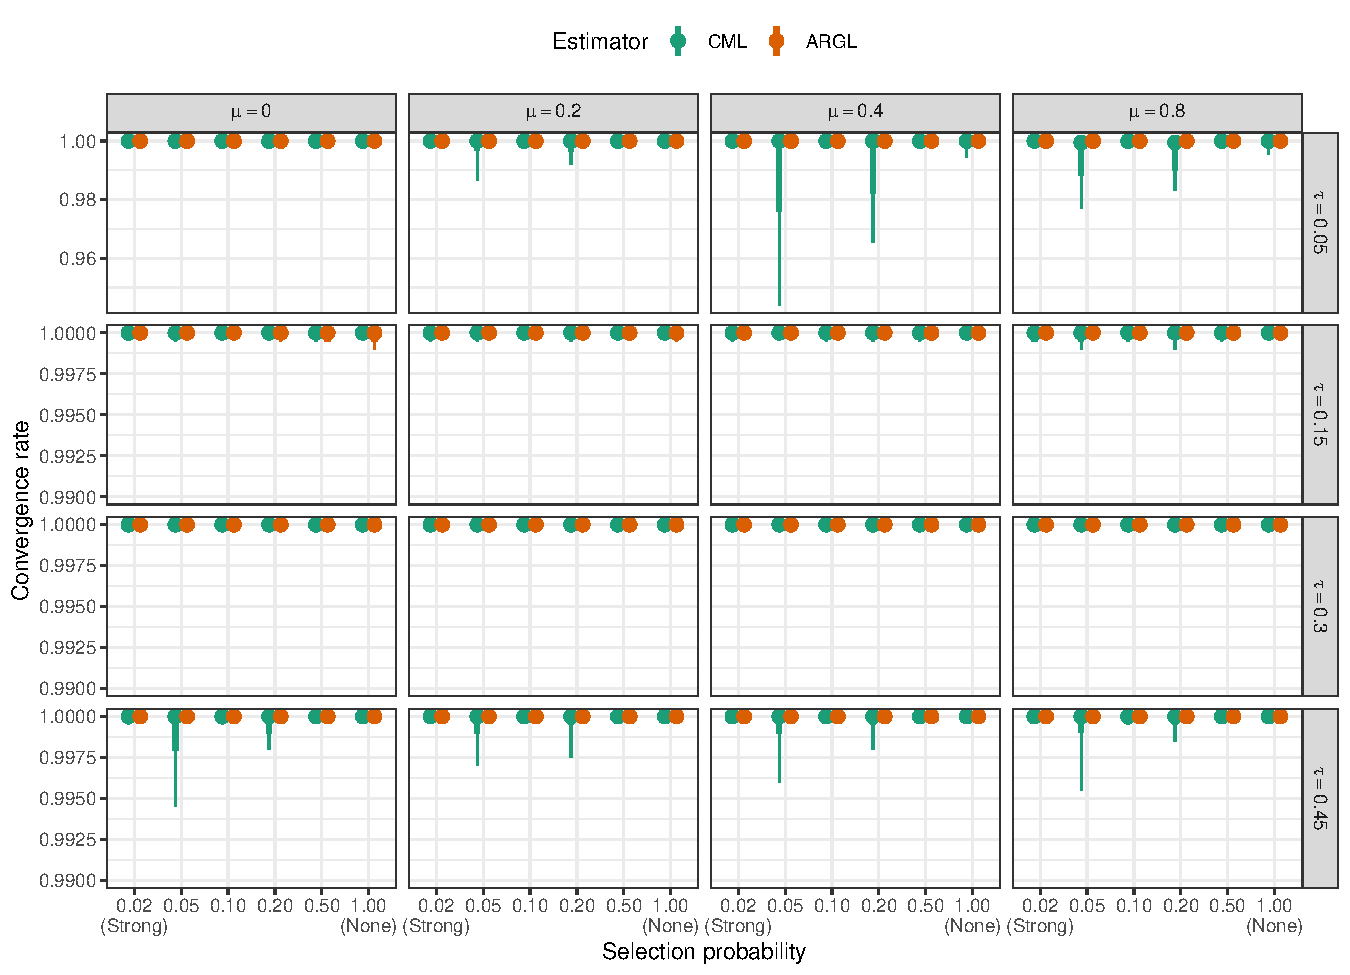
\includegraphics{step-function-selection-models-supplementary-materials_files/figure-latex/convergence-rates-1} \caption{Convergence rates of CML and ARGL estimators by selection probability, average SMD, and between-study heterogeneity. Points correspond to median convergence rates; thin lines correspond to range of convergence rates; thick lines correspond to inter-decile range.}\label{fig:convergence-rates}
\end{sidewaysfigure}

\begin{sidewaysfigure}
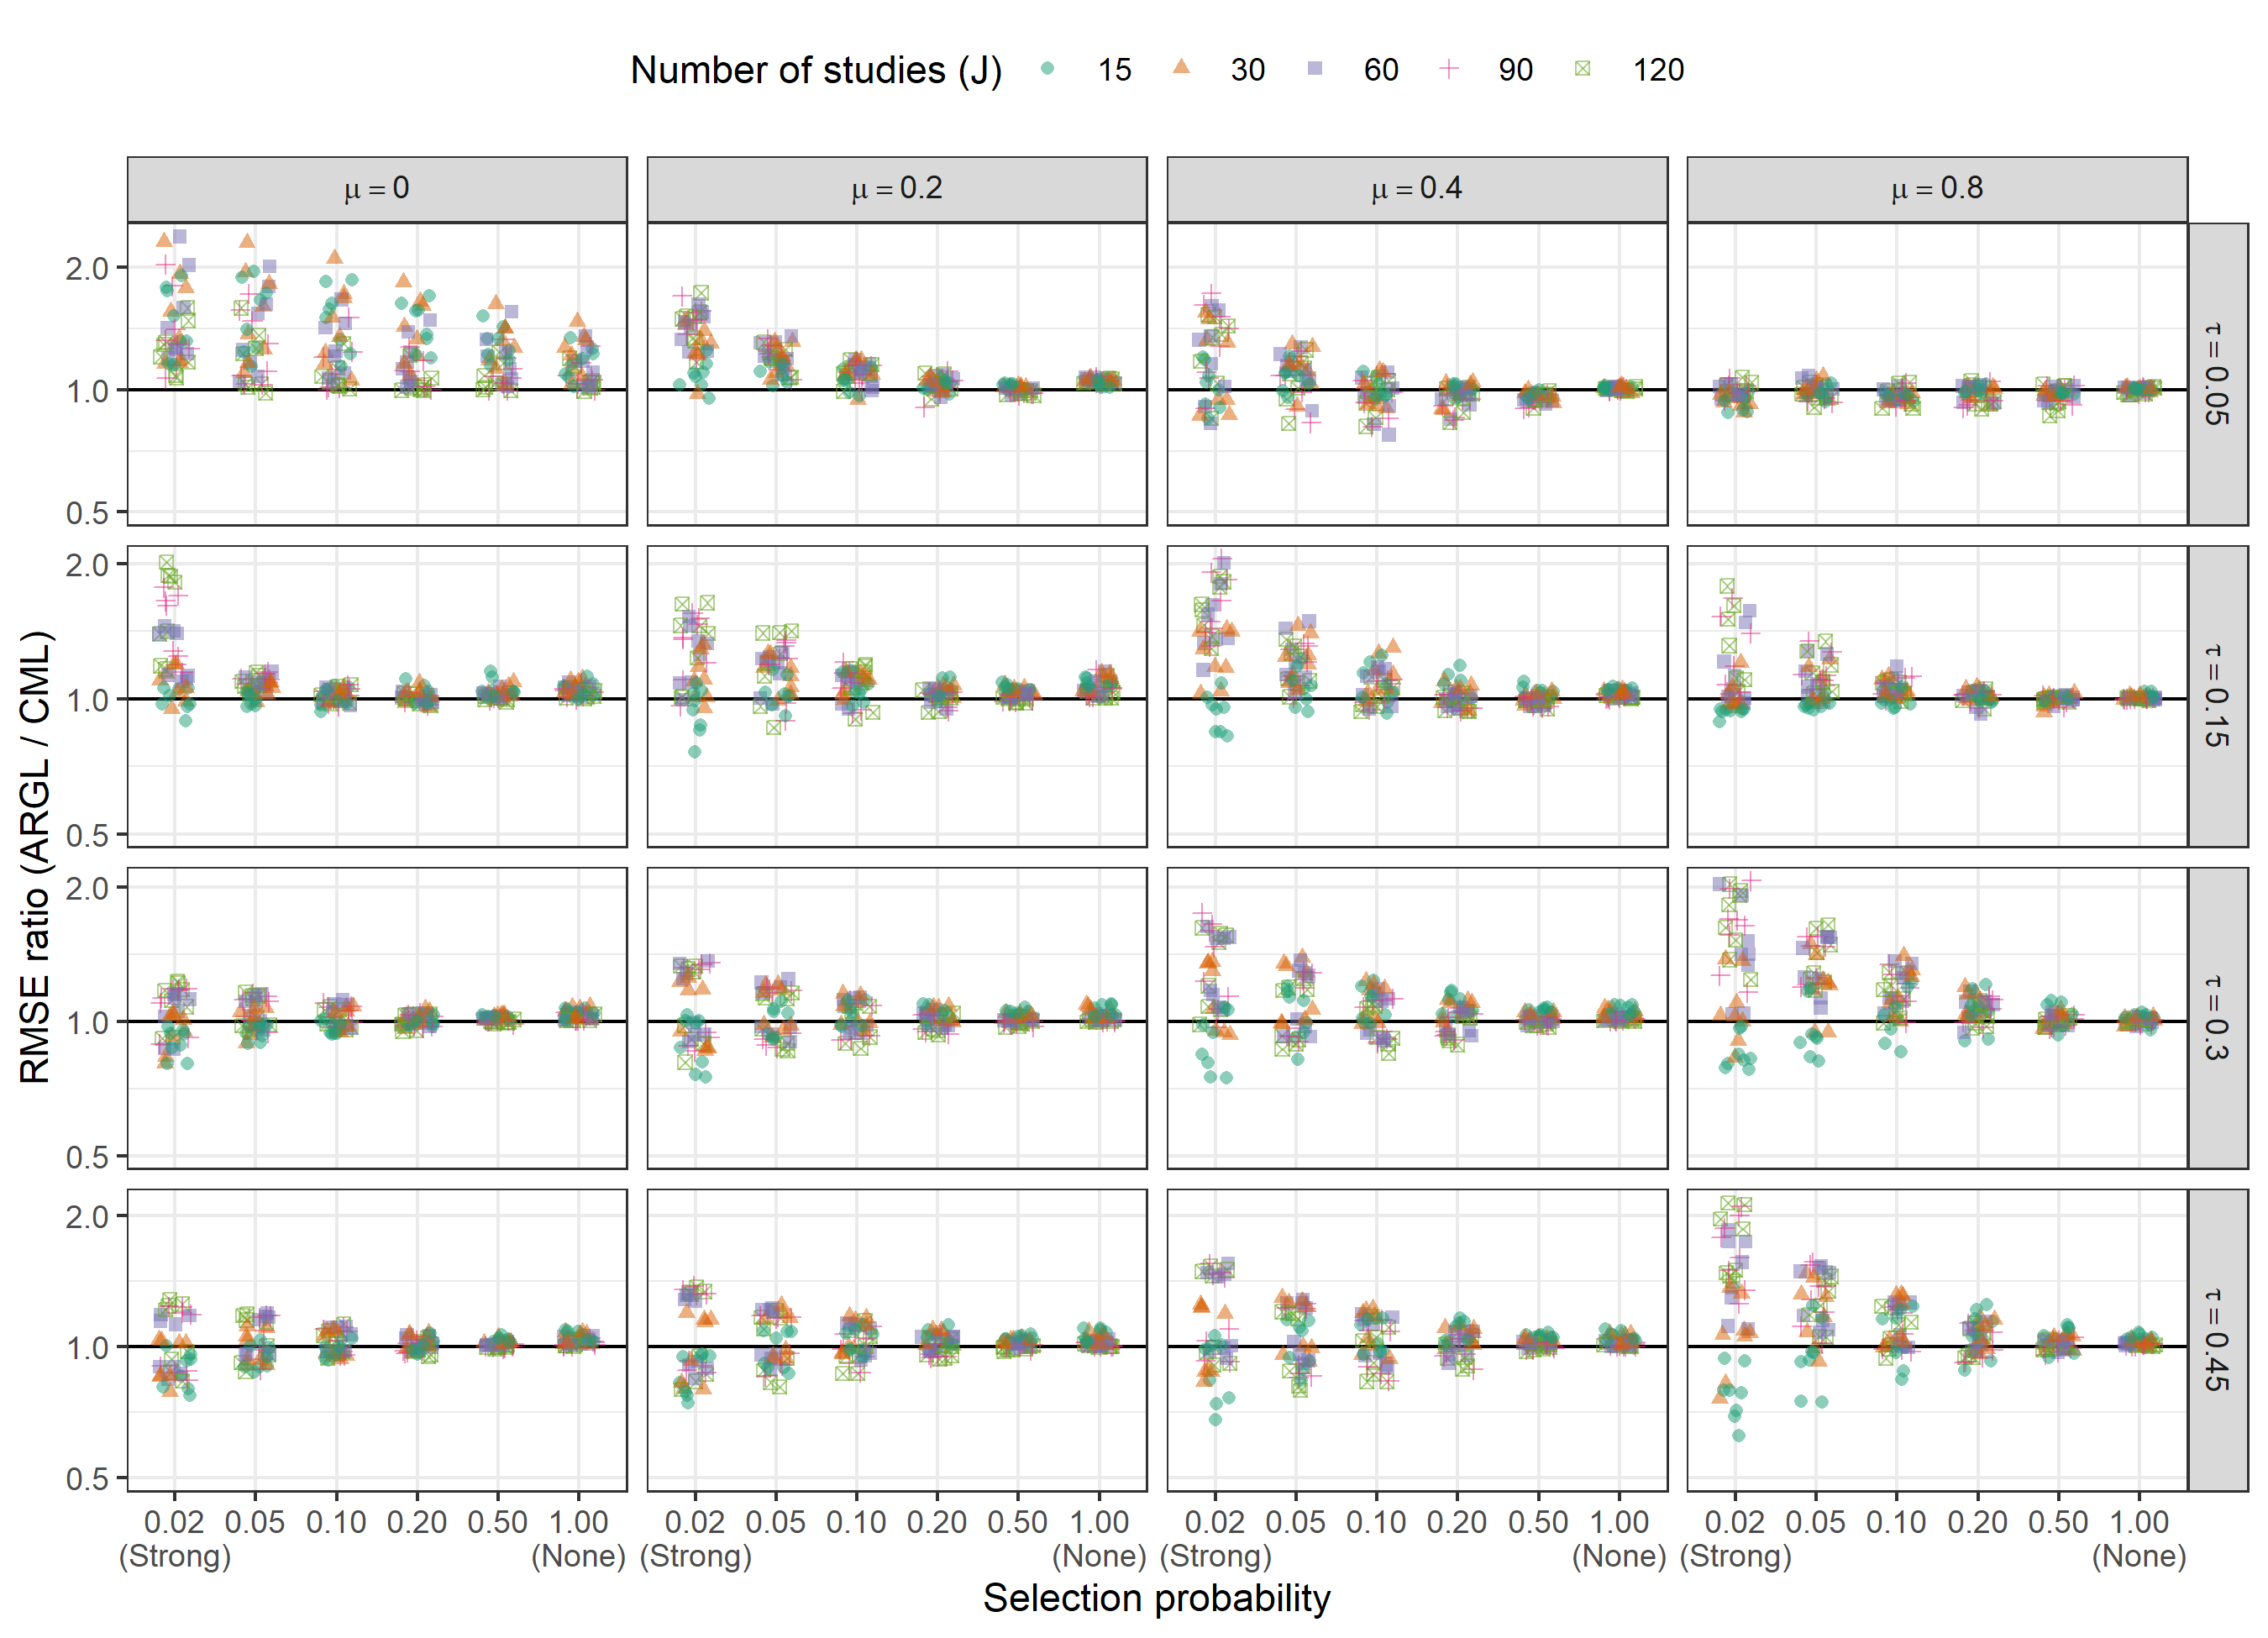
\includegraphics{step-function-selection-models-supplementary-materials_files/figure-latex/rmse-ARGL-CML-1} \caption{Ratio of root mean-squared error for ARGL estimator to root mean-squared error of CML estimator by selection probability, number of studies, average SMD, and between-study heterogeneity}\label{fig:rmse-ARGL-CML}
\end{sidewaysfigure}

\begin{sidewaysfigure}
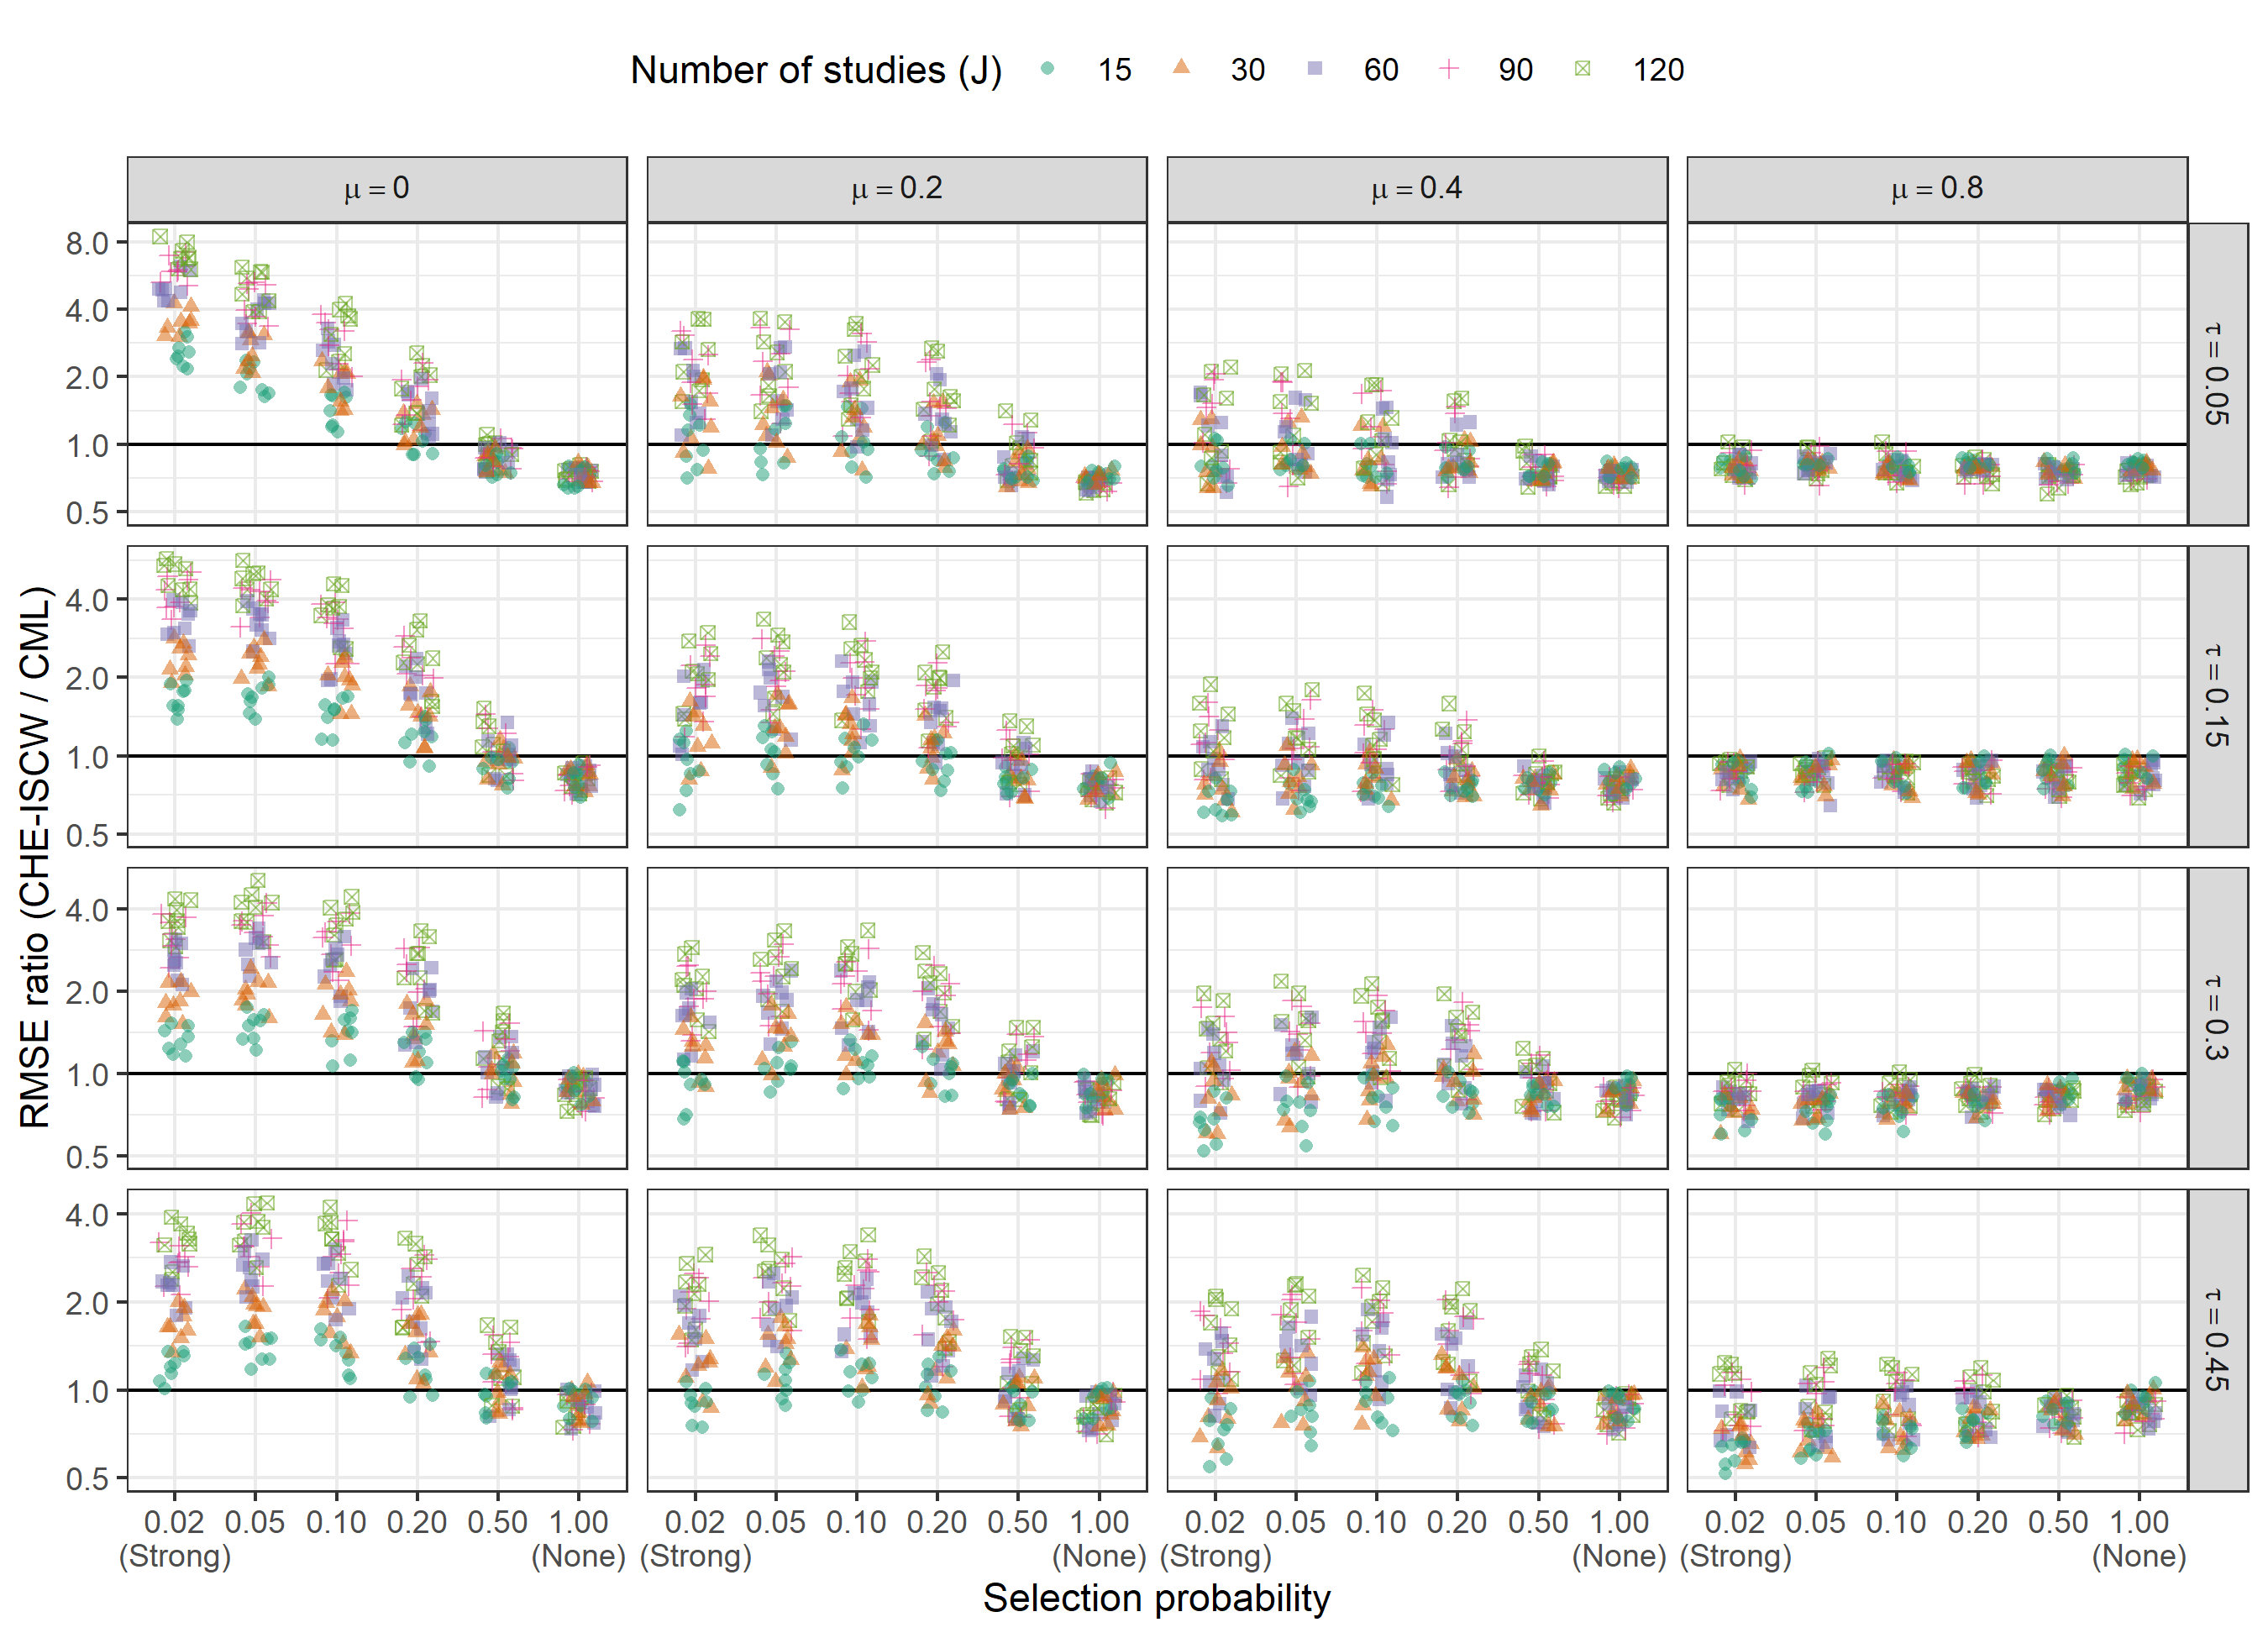
\includegraphics{step-function-selection-models-supplementary-materials_files/figure-latex/rmse-CHE-CML-1} \caption{Ratio of root mean-squared error for CHE-ISCW estimator to root mean-squared error of CML estimator by selection probability, number of studies, average SMD, and between-study heterogeneity}\label{fig:rmse-CHE-CML}
\end{sidewaysfigure}

\begin{sidewaysfigure}
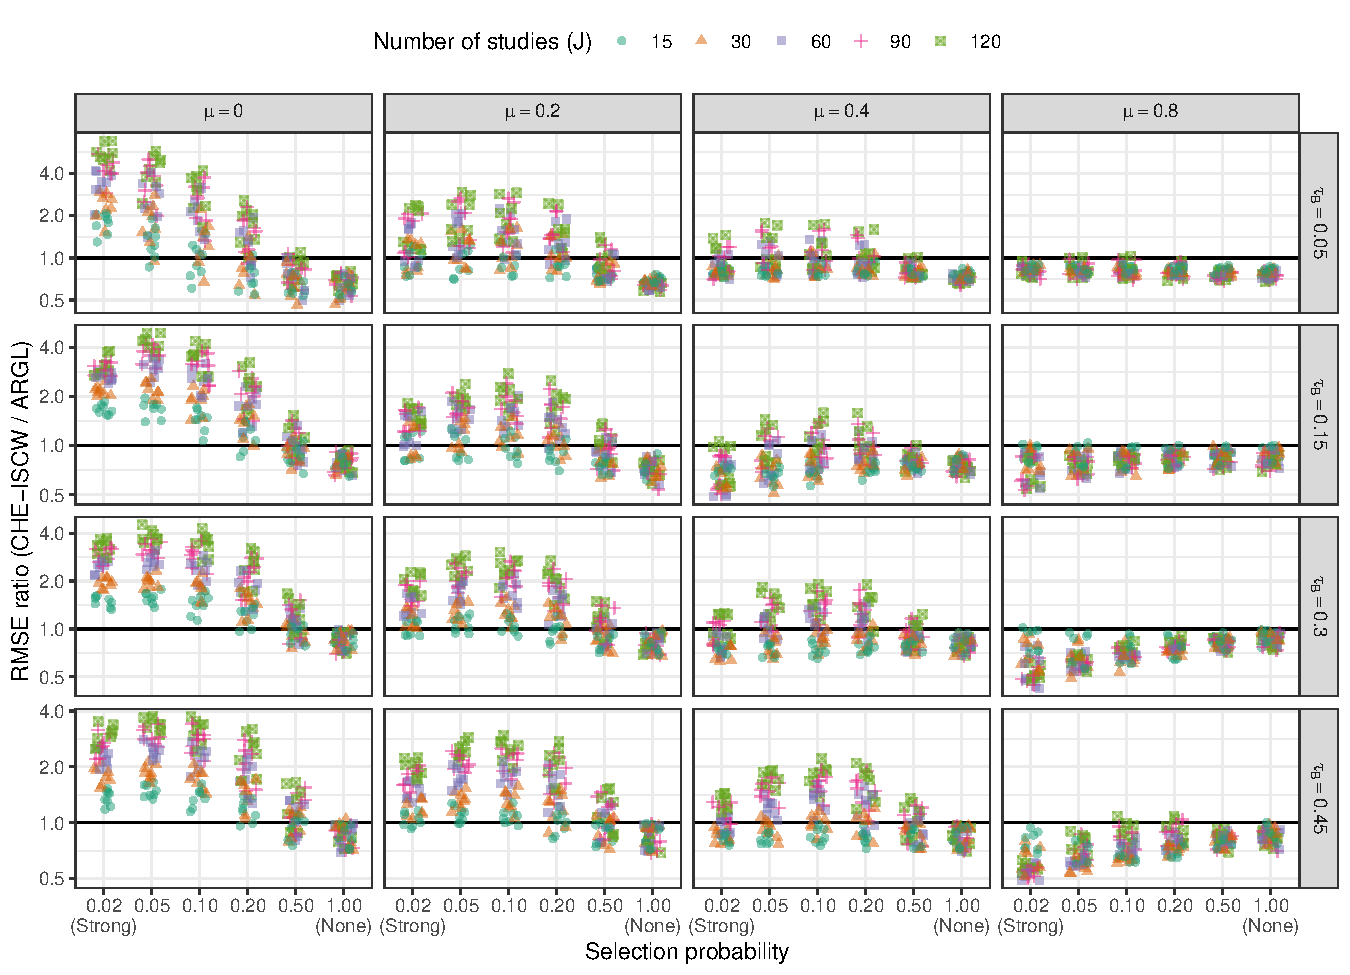
\includegraphics{step-function-selection-models-supplementary-materials_files/figure-latex/rmse-CHE-ARGL-1} \caption{Ratio of root mean-squared error for CHE-ISCW estimator to root mean-squared error of ARGL estimator by selection probability, number of studies, average SMD, and between-study heterogeneity}\label{fig:rmse-CHE-ARGL}
\end{sidewaysfigure}

\begin{sidewaysfigure}
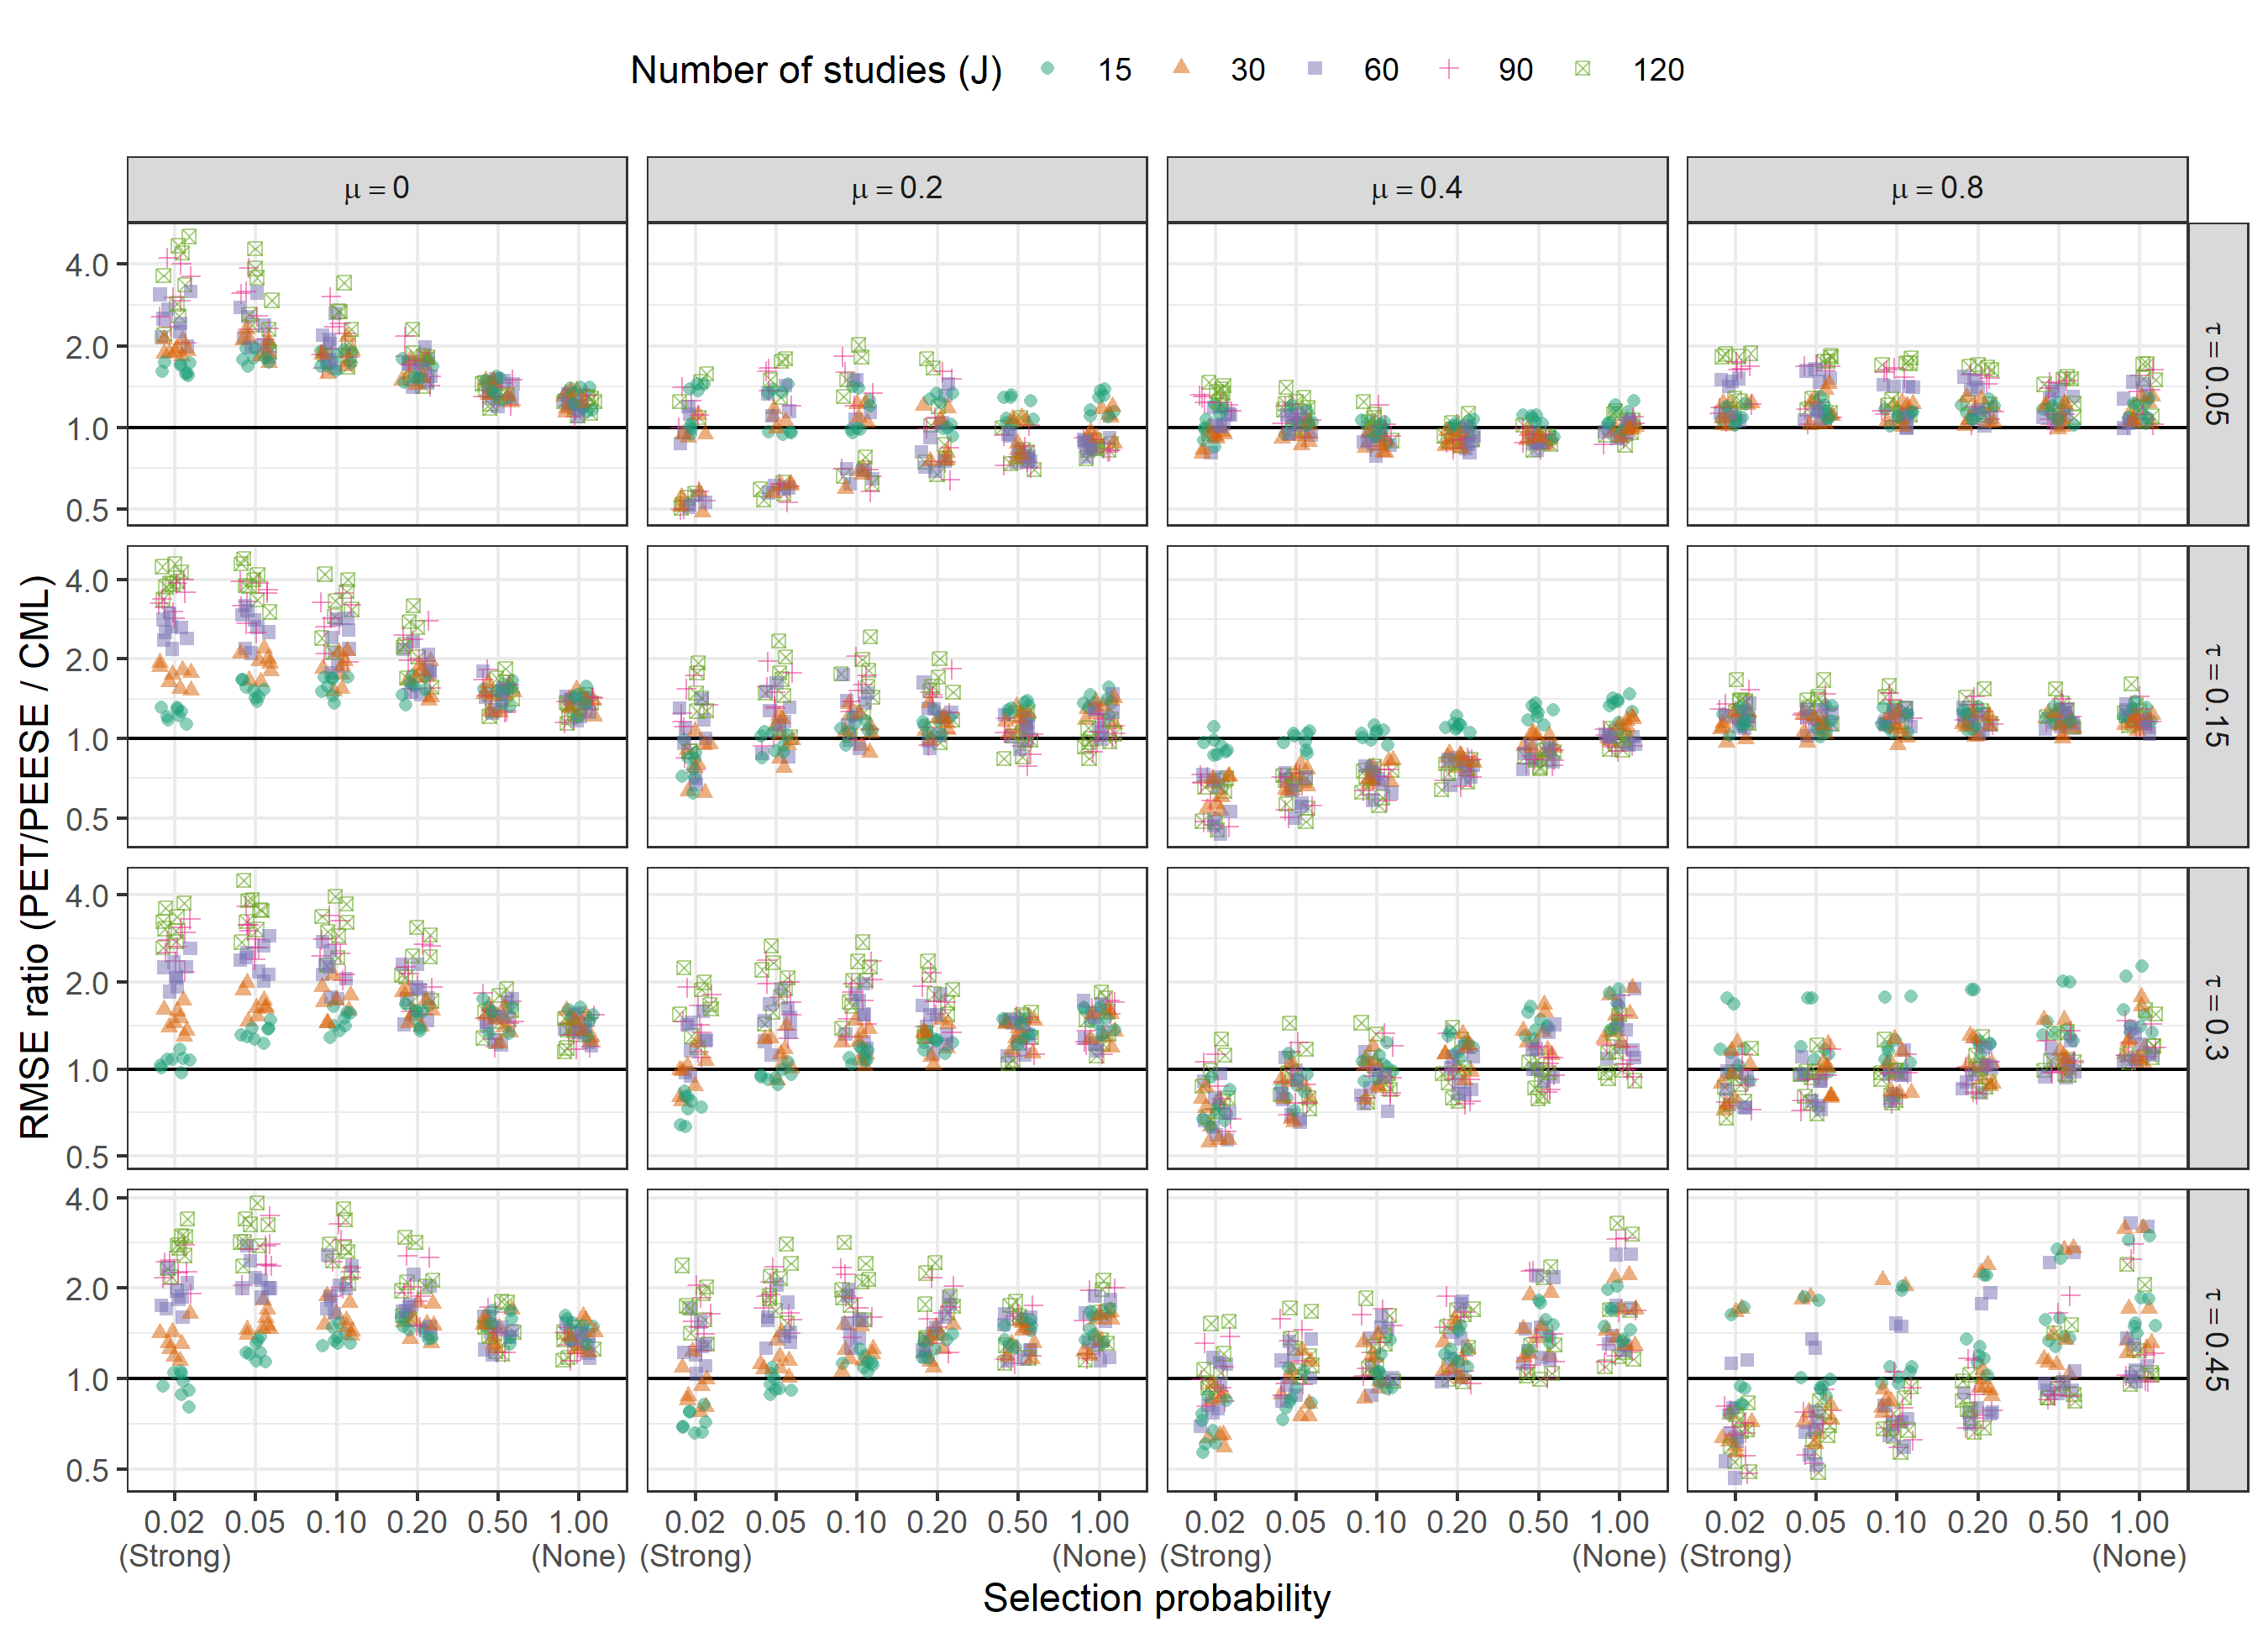
\includegraphics{step-function-selection-models-supplementary-materials_files/figure-latex/rmse-PET-CML-1} \caption{Ratio of root mean-squared error for PET/PEESE estimator to root mean-squared error of CML estimator by selection probability, number of studies, average SMD, and between-study heterogeneity}\label{fig:rmse-PET-CML}
\end{sidewaysfigure}

\begin{sidewaysfigure}
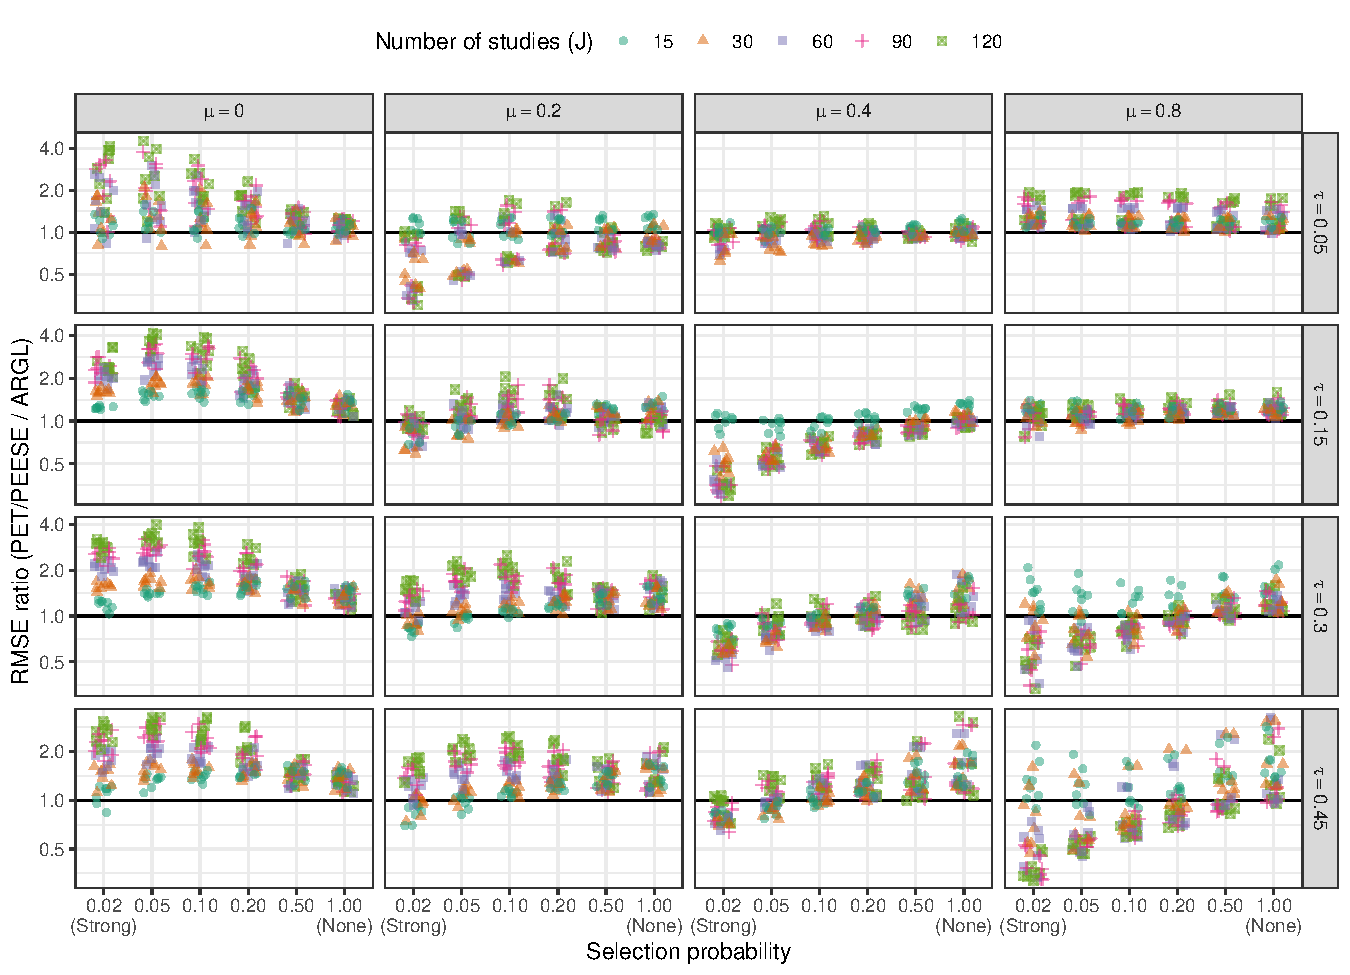
\includegraphics{step-function-selection-models-supplementary-materials_files/figure-latex/rmse-PET-ARGL-1} \caption{Ratio of root mean-squared error for PET/PEESE estimator to root mean-squared error of ARGL estimator by selection probability, number of studies, average SMD, and between-study heterogeneity}\label{fig:rmse-PET-ARGL}
\end{sidewaysfigure}

\begin{sidewaysfigure}
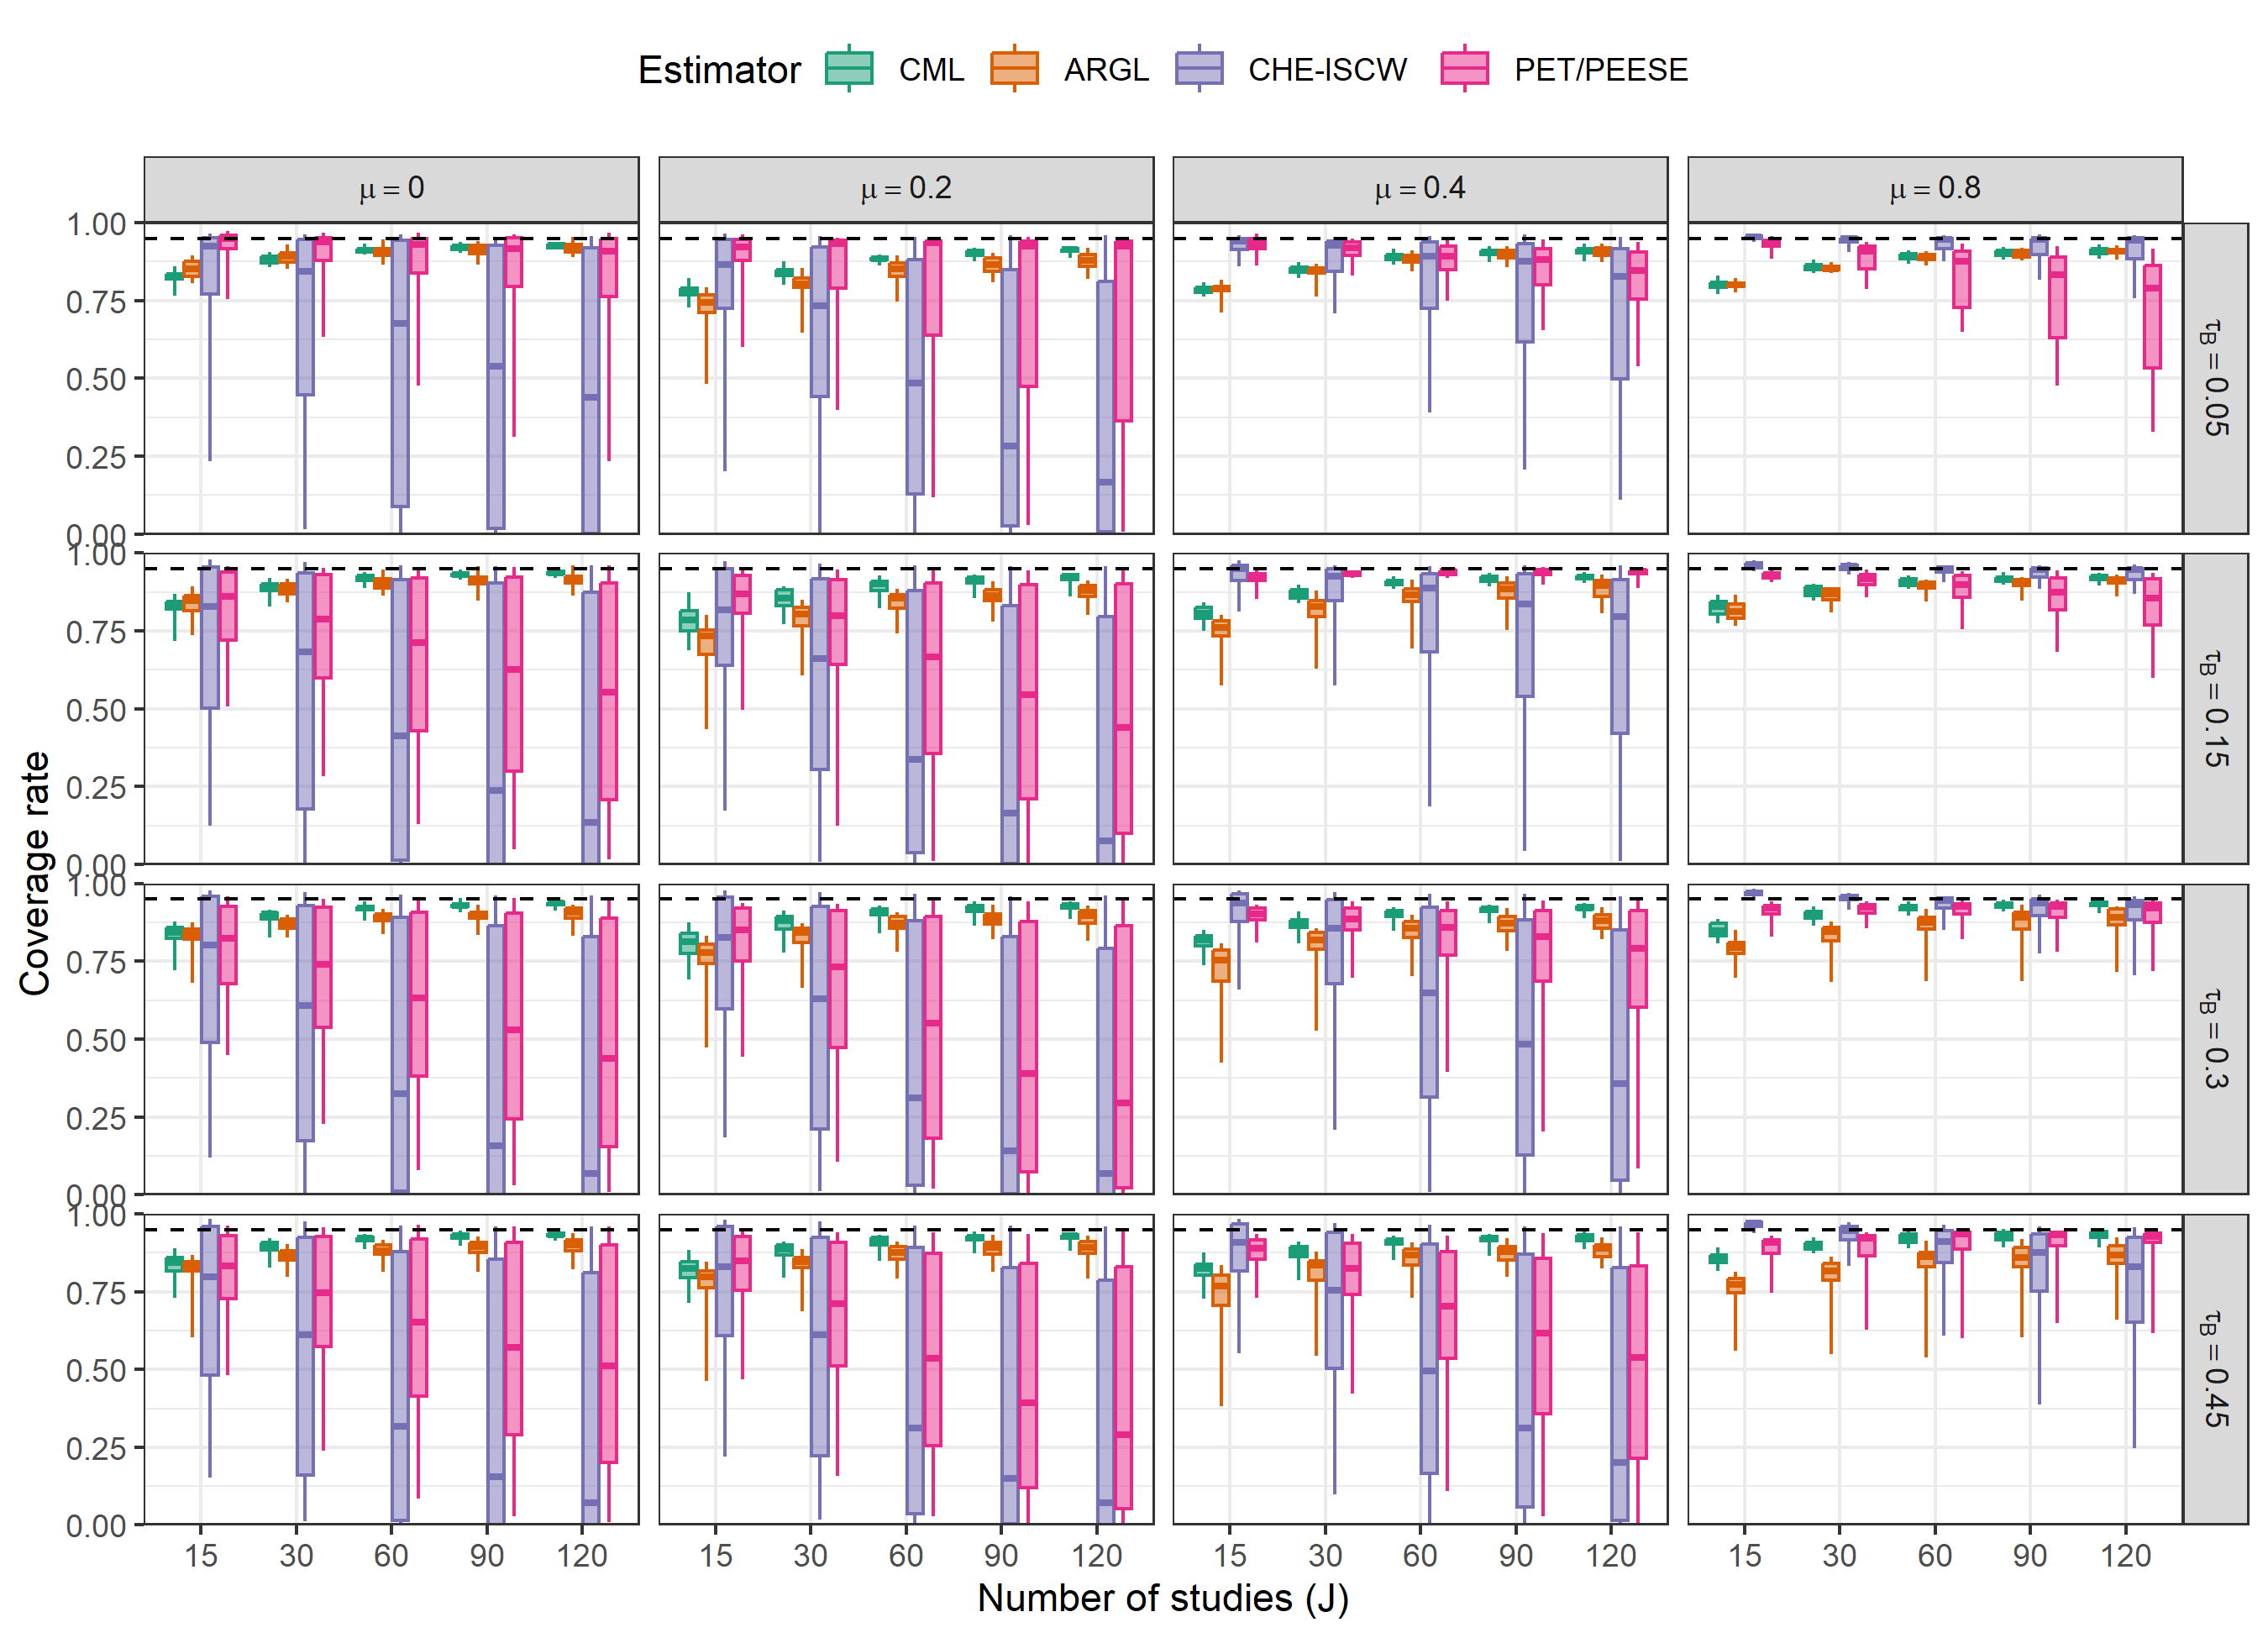
\includegraphics{step-function-selection-models-supplementary-materials_files/figure-latex/comparison-coverage-full-1} \caption{Coverage levels of confidence intervals based for average effect size based on cluster-robust variance approximations, by number of studies, average SMD, and between-study heterogeneity. Dashed lines correspond to the nominal confidence level of 0.95.}\label{fig:comparison-coverage-full}
\end{sidewaysfigure}

\begin{sidewaysfigure}
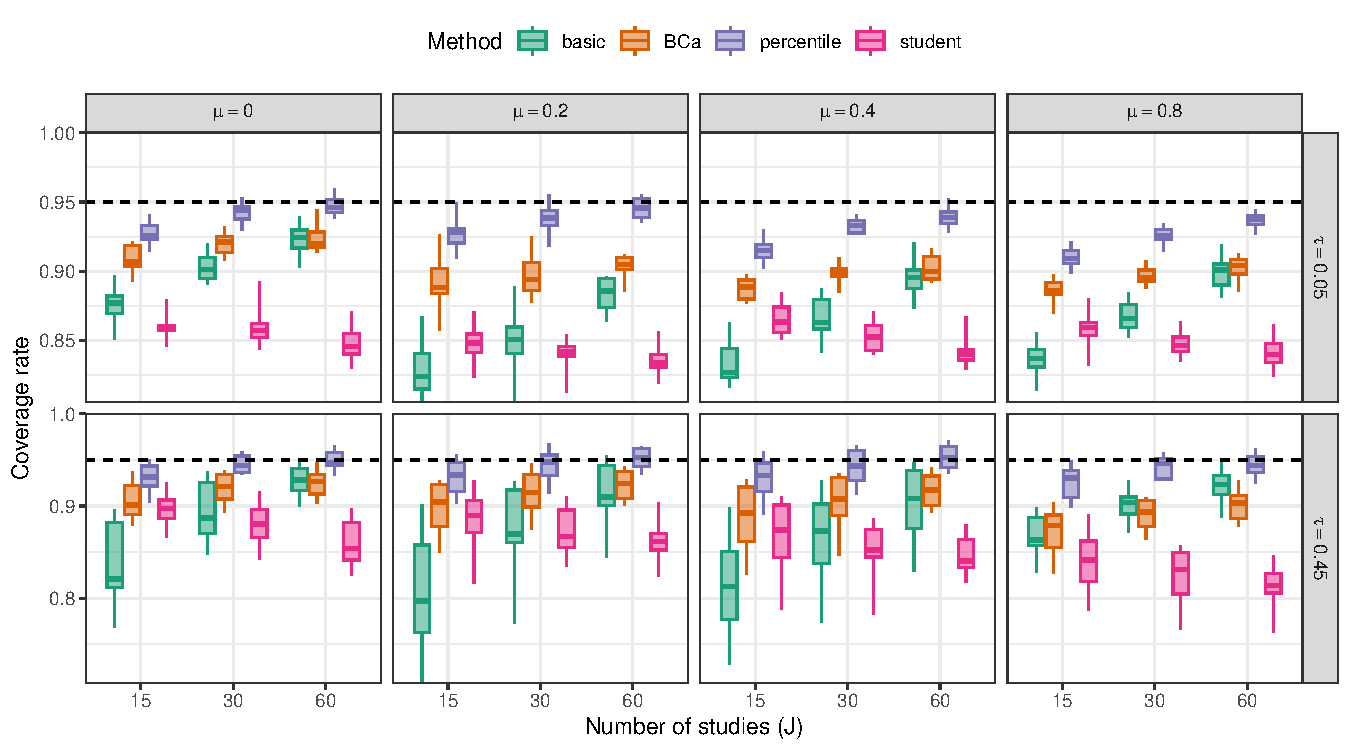
\includegraphics{step-function-selection-models-supplementary-materials_files/figure-latex/CML-coverage-two-stage-1} \caption{Coverage levels of two-stage bootstrap confidence intervals based on the CML estimator of average effect size by number of studies, average SMD, and between-study heterogeneity. Dashed lines correspond to the nominal confidence level of 0.95.}\label{fig:CML-coverage-two-stage}
\end{sidewaysfigure}

\begin{sidewaysfigure}
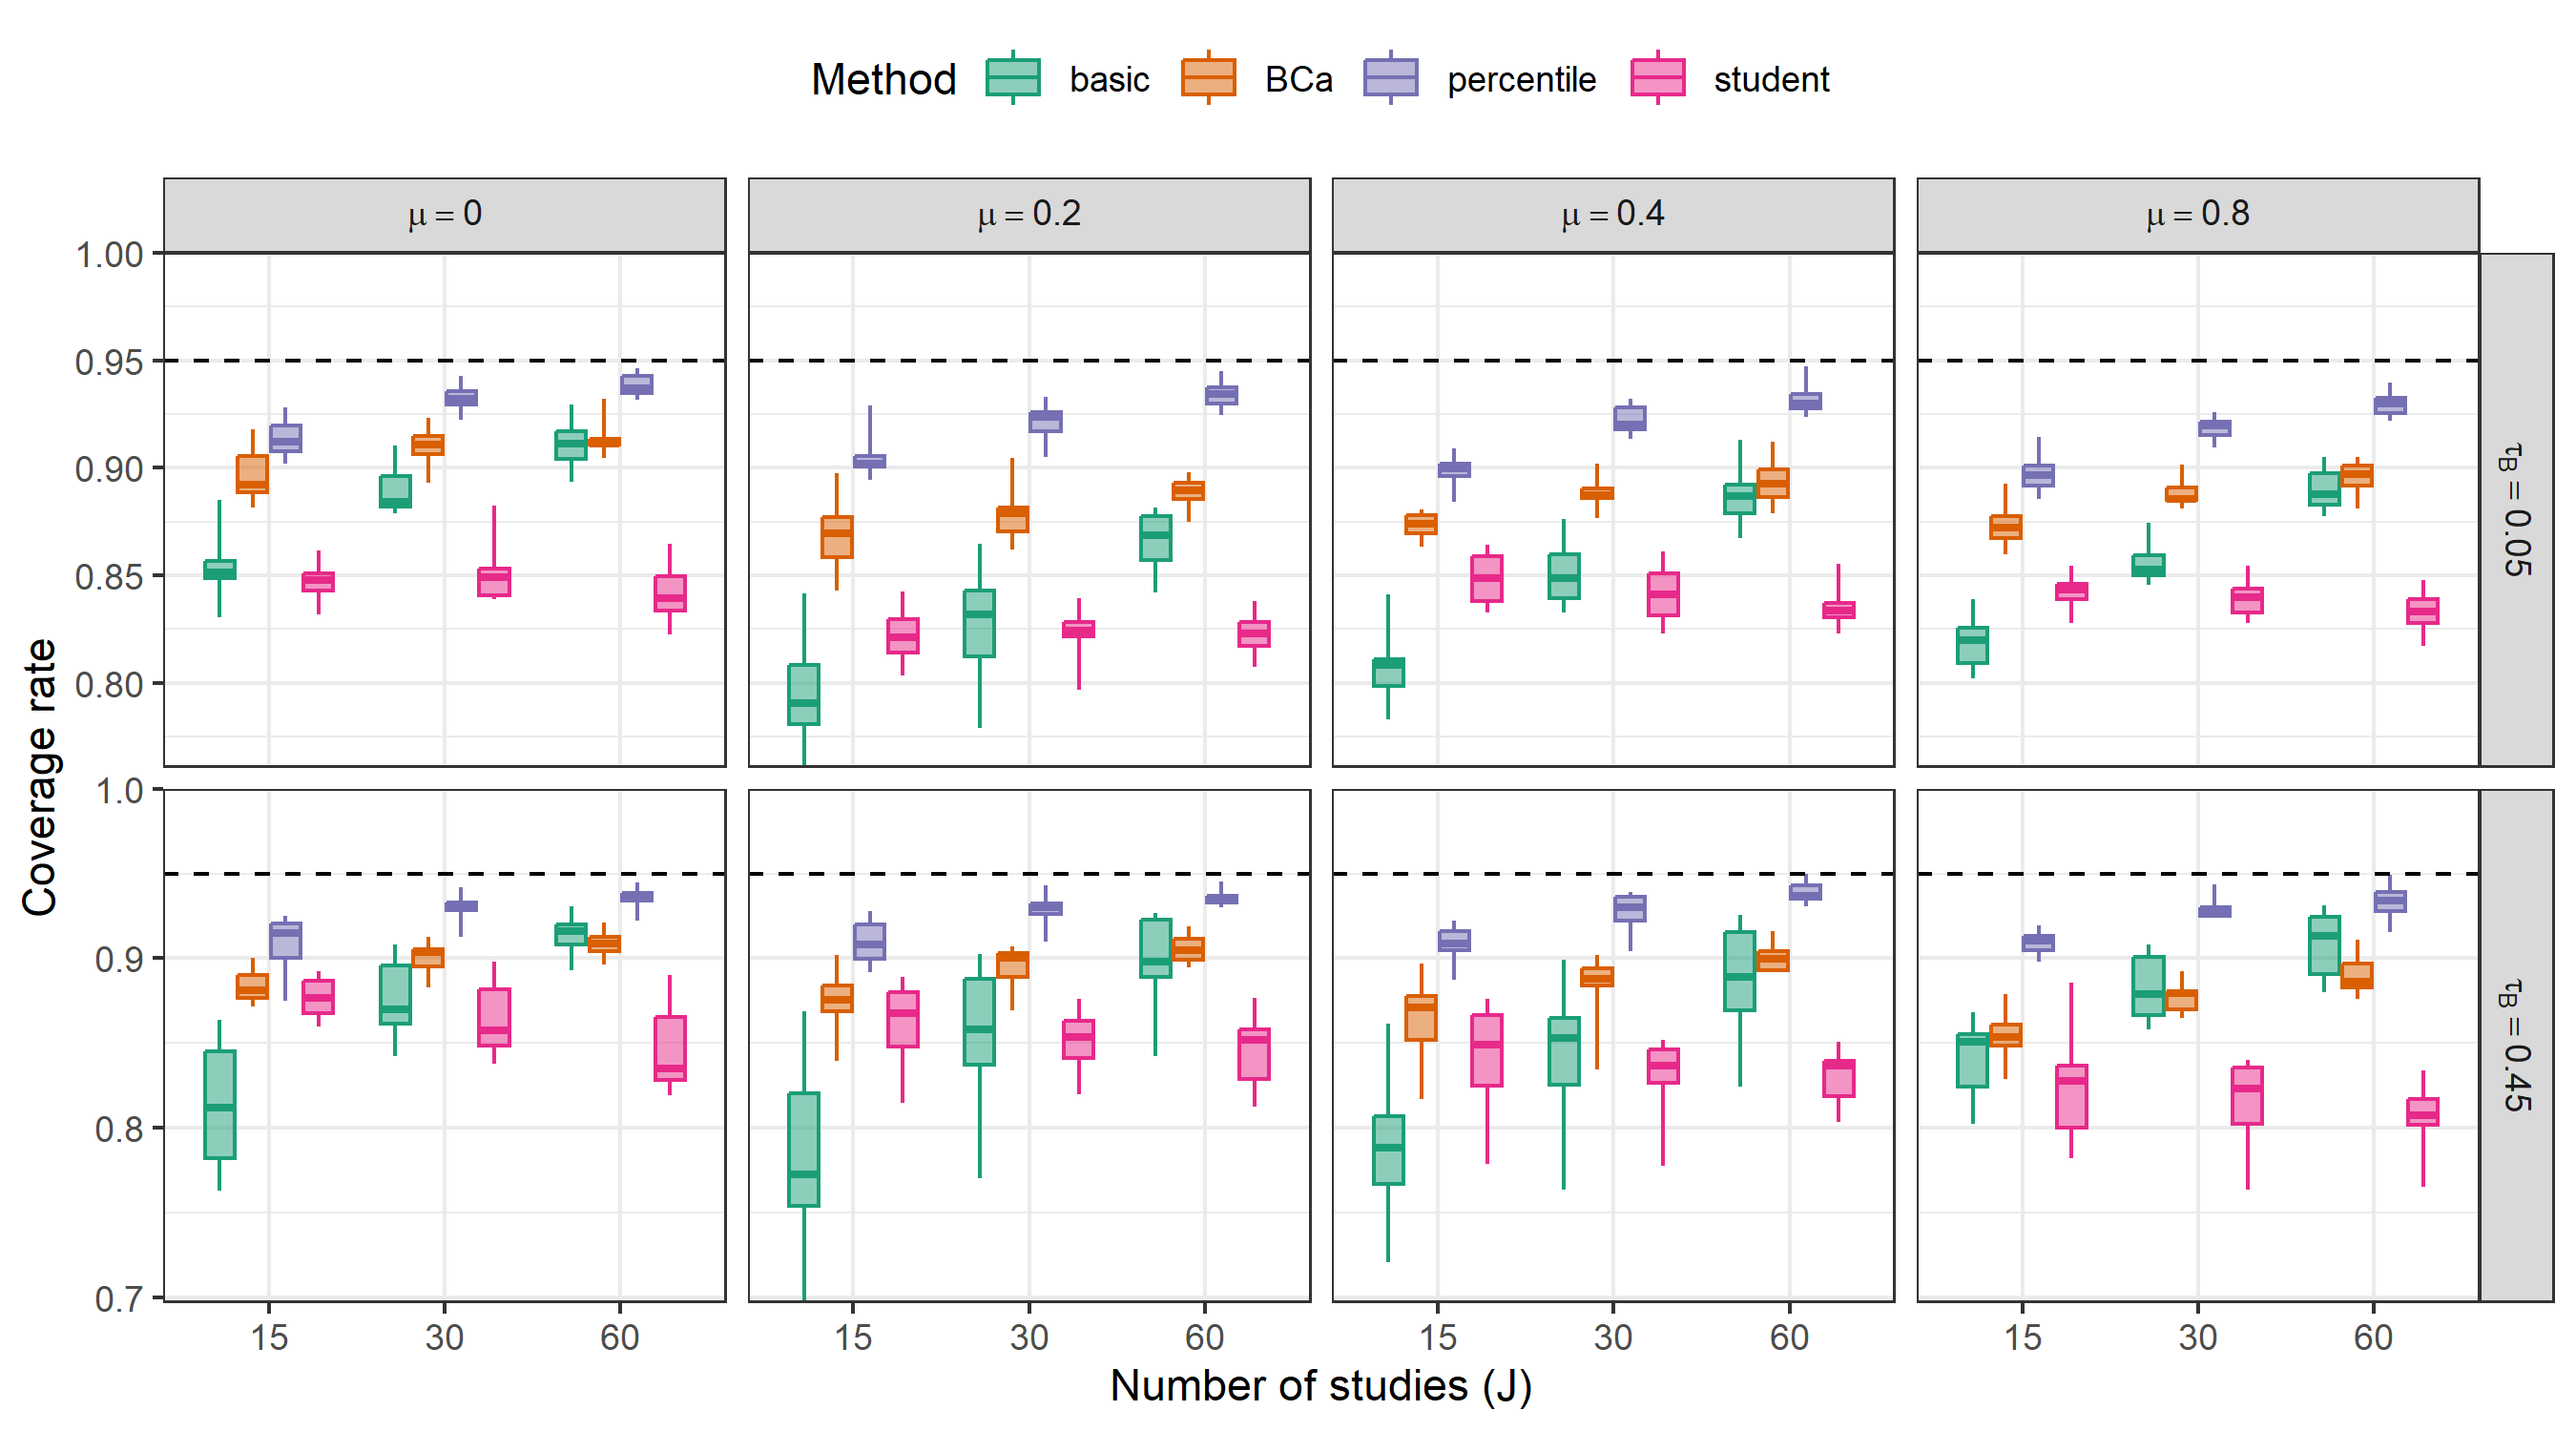
\includegraphics{step-function-selection-models-supplementary-materials_files/figure-latex/CML-coverage-multinomial-1} \caption{Coverage levels of multinomial bootstrap confidence intervals based on the CML estimator of average effect size by number of studies, average SMD, and between-study heterogeneity. Dashed lines correspond to the nominal confidence level of 0.95.}\label{fig:CML-coverage-multinomial}
\end{sidewaysfigure}

\begin{sidewaysfigure}
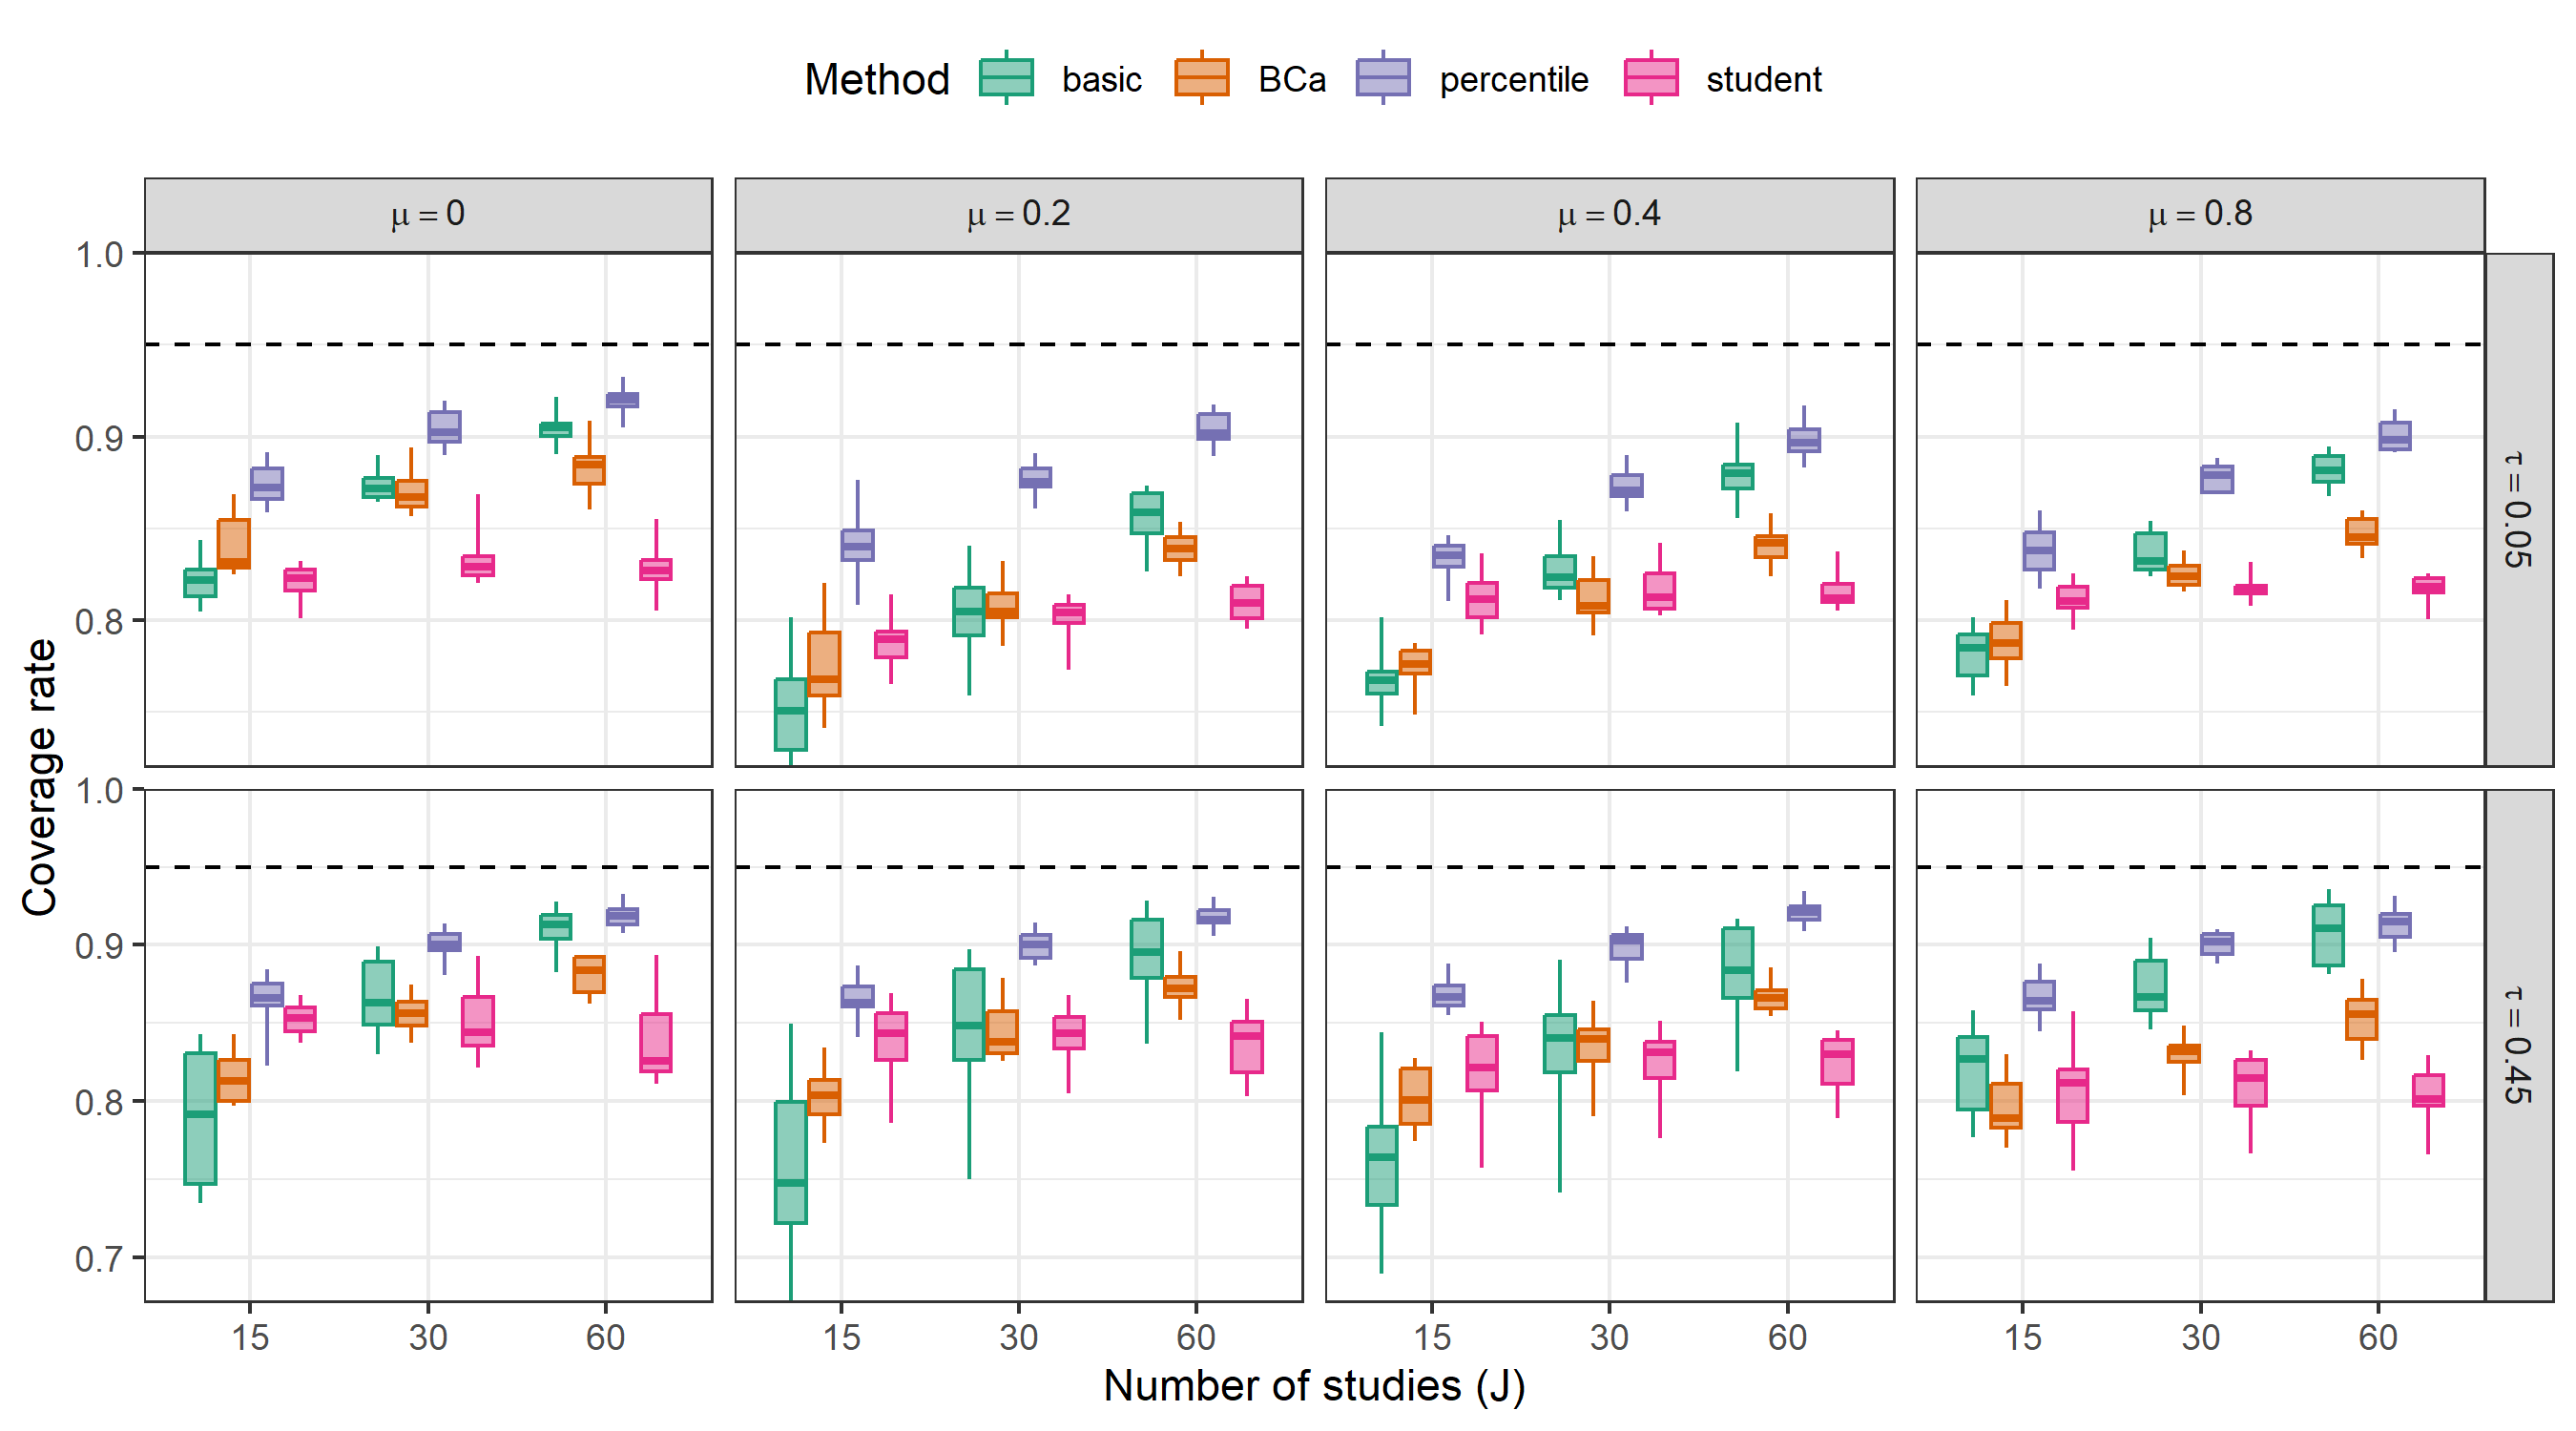
\includegraphics{step-function-selection-models-supplementary-materials_files/figure-latex/CML-coverage-exponential-1} \caption{Coverage levels of fractional random weight bootstrap confidence intervals based on the CML estimator of average effect size by number of studies, average SMD, and between-study heterogeneity. Dashed lines correspond to the nominal confidence level of 0.95.}\label{fig:CML-coverage-exponential}
\end{sidewaysfigure}

\begin{sidewaysfigure}
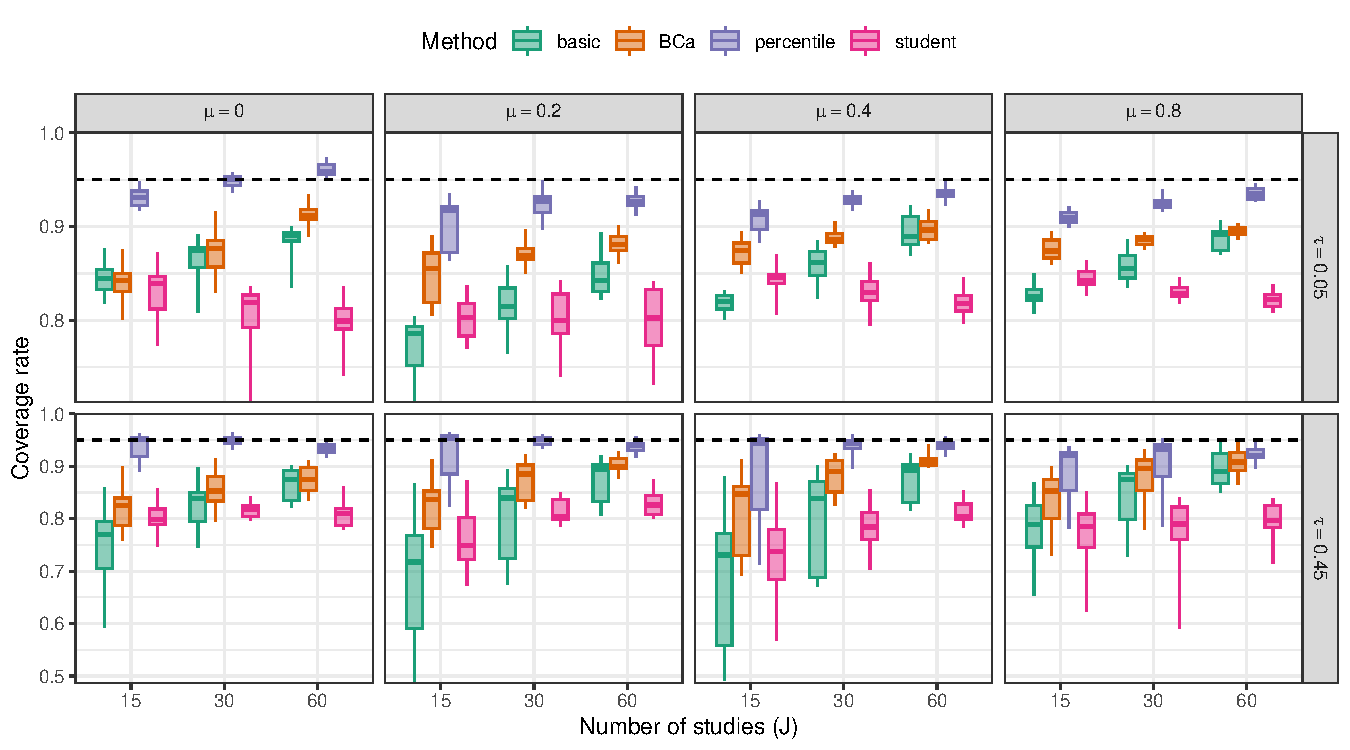
\includegraphics{step-function-selection-models-supplementary-materials_files/figure-latex/ARGL-coverage-two-stage-1} \caption{Coverage levels of two-stage bootstrap confidence intervals based on the ARGL estimator of average effect size by number of studies, average SMD, and between-study heterogeneity. Dashed lines correspond to the nominal confidence level of 0.95.}\label{fig:ARGL-coverage-two-stage}
\end{sidewaysfigure}

\begin{sidewaysfigure}
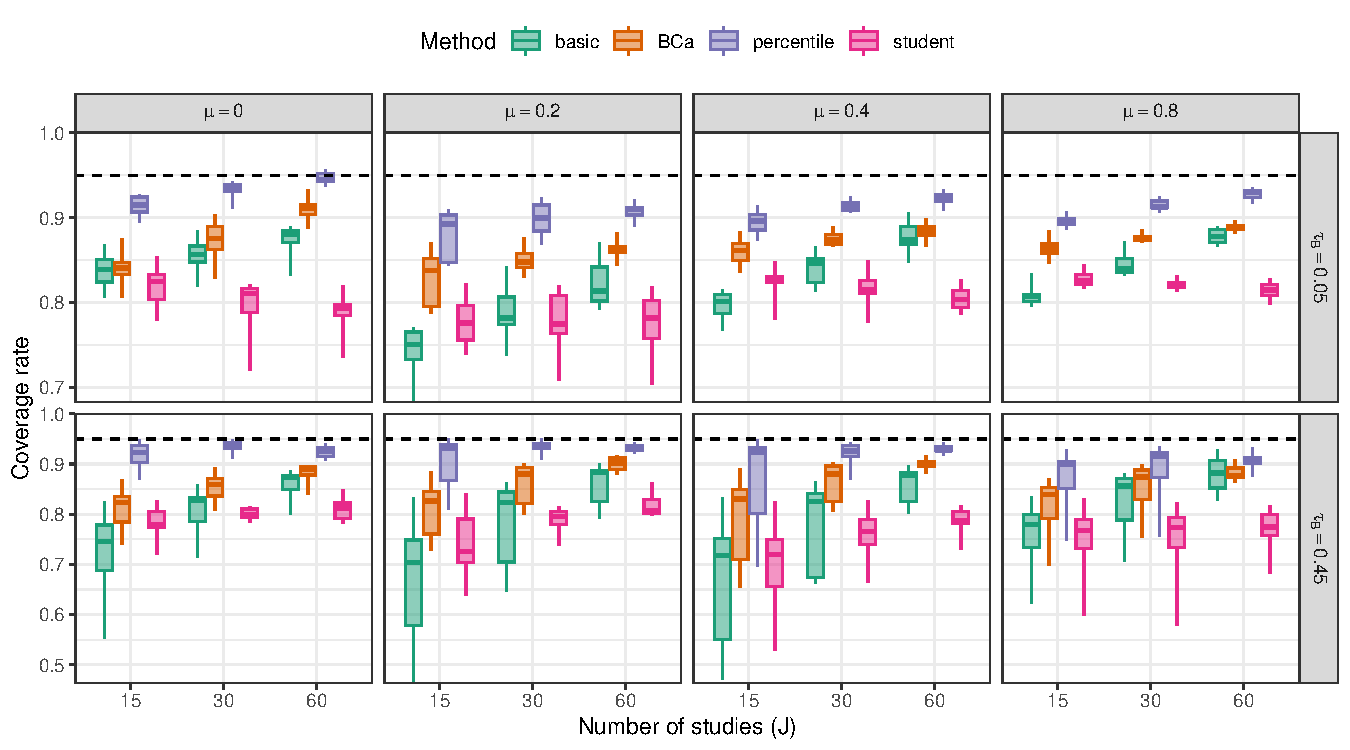
\includegraphics{step-function-selection-models-supplementary-materials_files/figure-latex/ARGL-coverage-multinomial-1} \caption{Coverage levels of multinomial bootstrap confidence intervals based on the ARGL estimator of average effect size by number of studies, average SMD, and between-study heterogeneity. Dashed lines correspond to the nominal confidence level of 0.95.}\label{fig:ARGL-coverage-multinomial}
\end{sidewaysfigure}

\begin{sidewaysfigure}
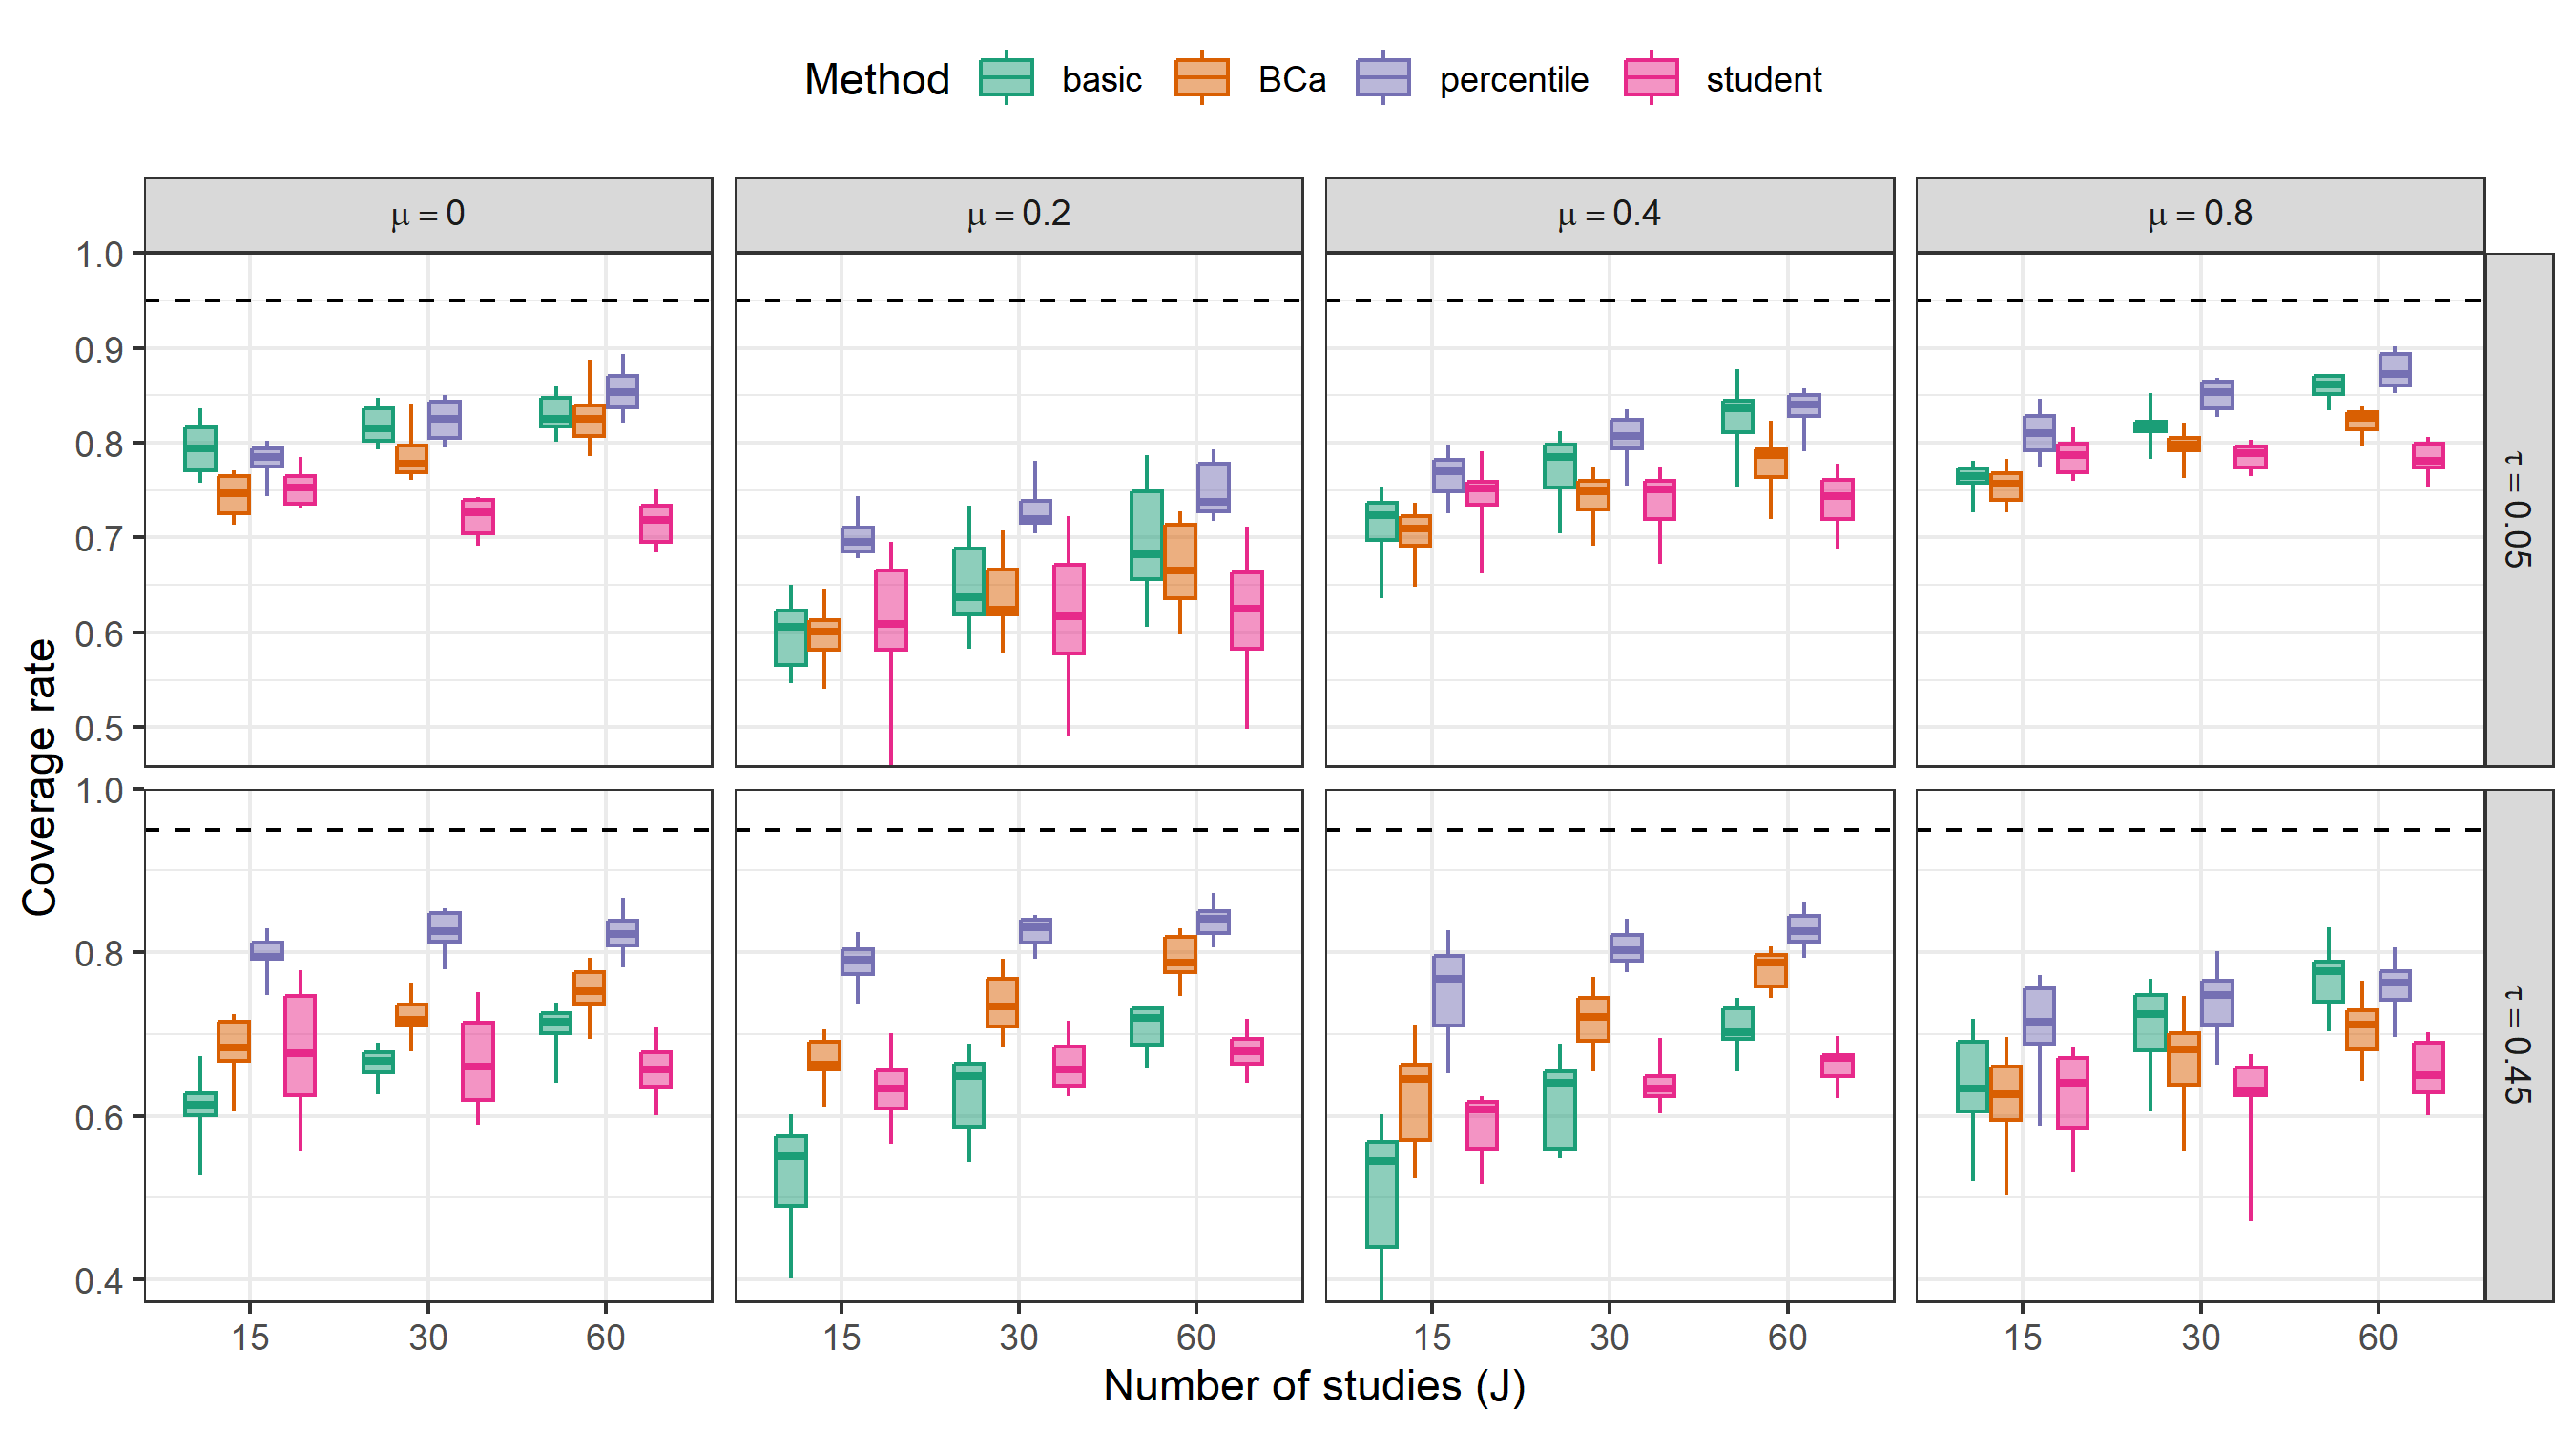
\includegraphics{step-function-selection-models-supplementary-materials_files/figure-latex/ARGL-coverage-exponential-1} \caption{Coverage levels of fractional random weight bootstrap confidence intervals based on the ARGL estimator of average effect size by number of studies, average SMD, and between-study heterogeneity. Dashed lines correspond to the nominal confidence level of 0.95.}\label{fig:ARGL-coverage-exponential}
\end{sidewaysfigure}

\section{\texorpdfstring{Additional simulation results for estimators of log-heterogeneity \((\gamma)\)}{Additional simulation results for estimators of log-heterogeneity (\textbackslash gamma)}}\label{gamma-simulation-results}

\begin{sidewaysfigure}
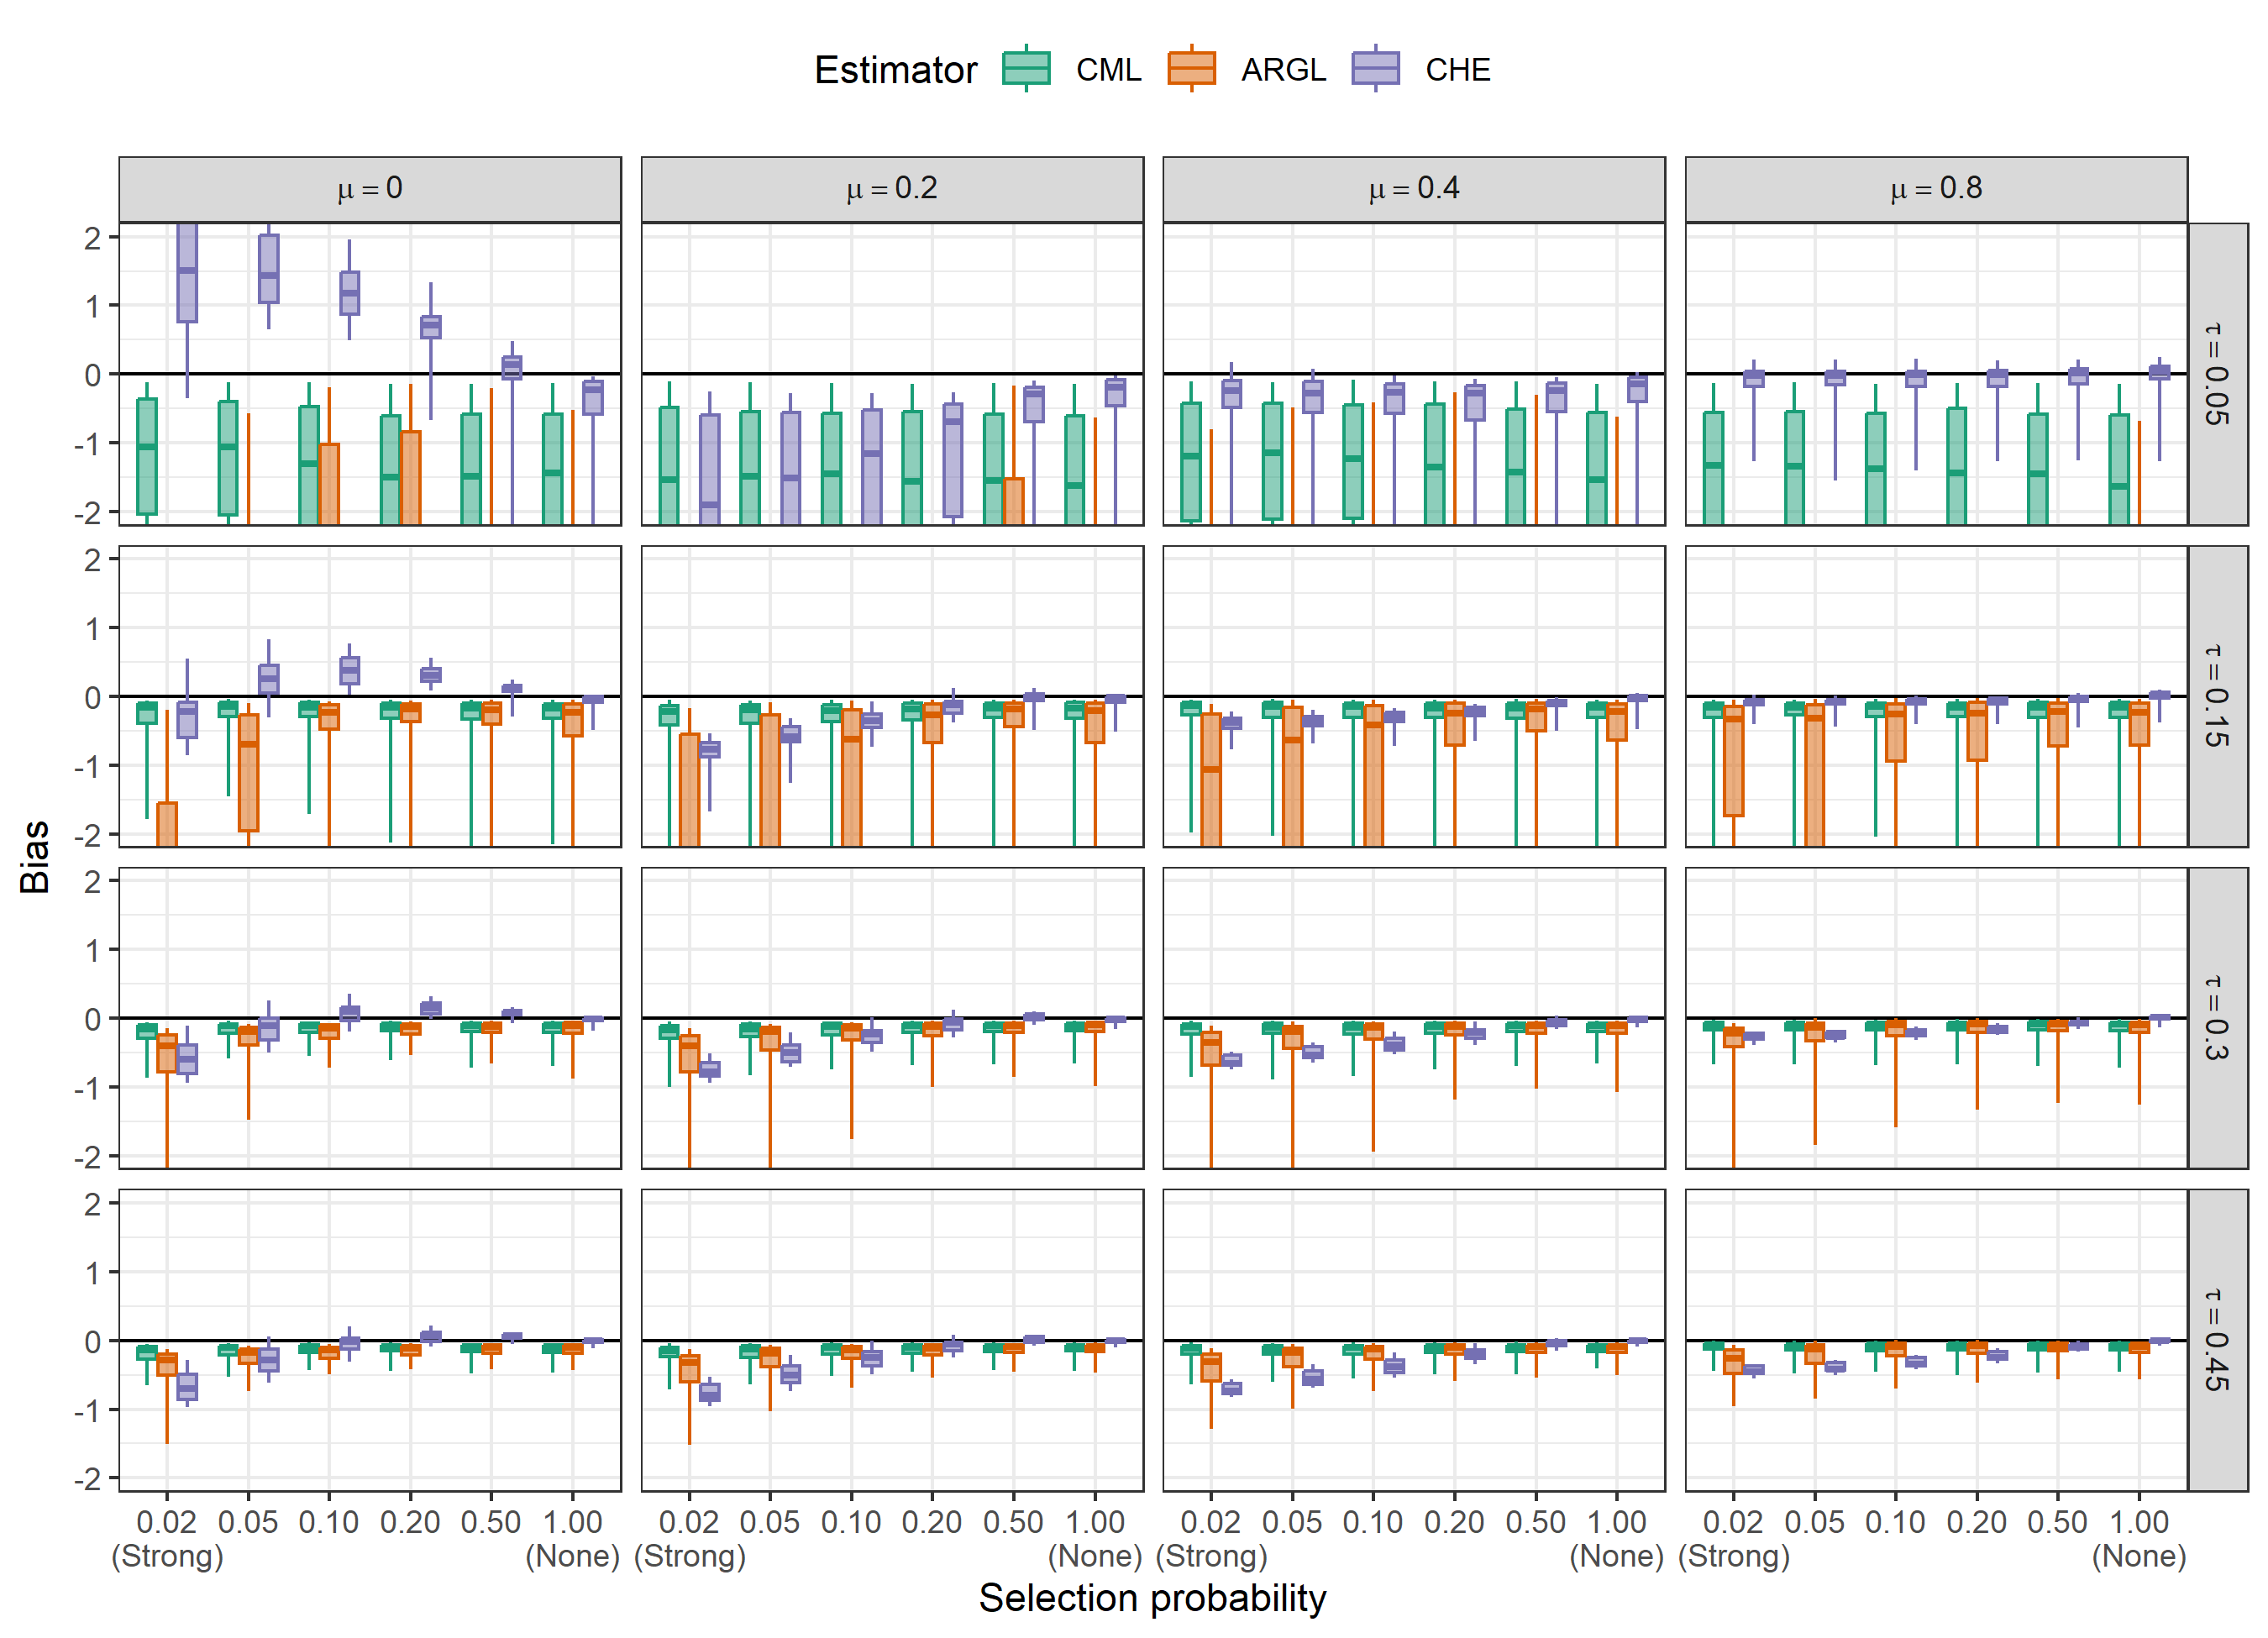
\includegraphics{step-function-selection-models-supplementary-materials_files/figure-latex/heterogeneity-bias-1} \caption{Bias for estimators of log-heterogeneity by selection probability, average SMD, and between-study heterogeneity}\label{fig:heterogeneity-bias}
\end{sidewaysfigure}

\begin{sidewaysfigure}
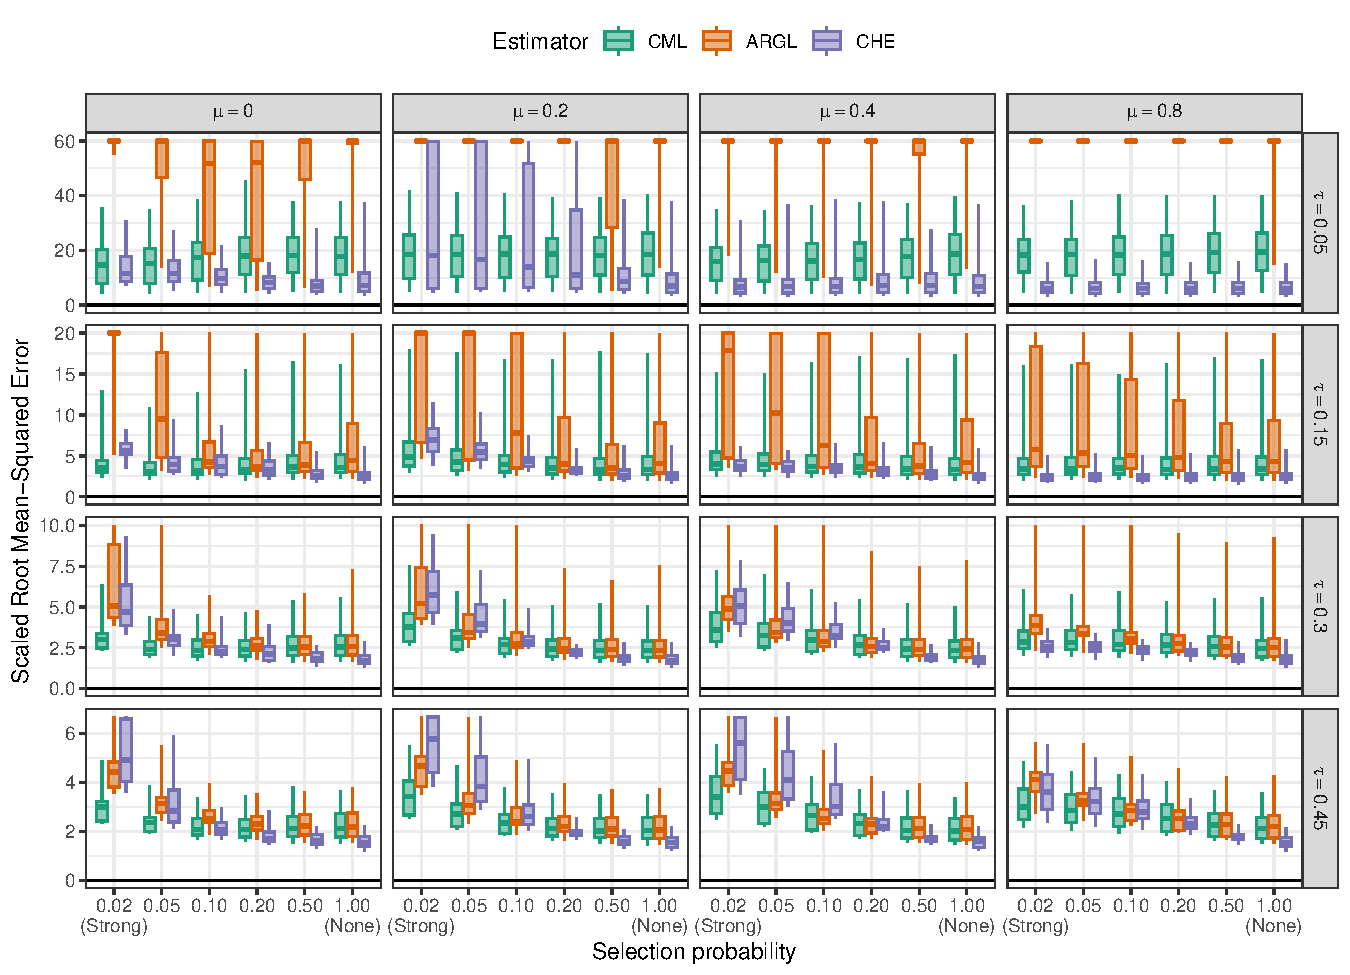
\includegraphics{step-function-selection-models-supplementary-materials_files/figure-latex/heterogeneity-rmse-1} \caption{Scaled root mean-squared error for estimators of log-heterogeneity by selection probability, average SMD, and between-study heterogeneity}\label{fig:heterogeneity-rmse}
\end{sidewaysfigure}

\begin{sidewaysfigure}
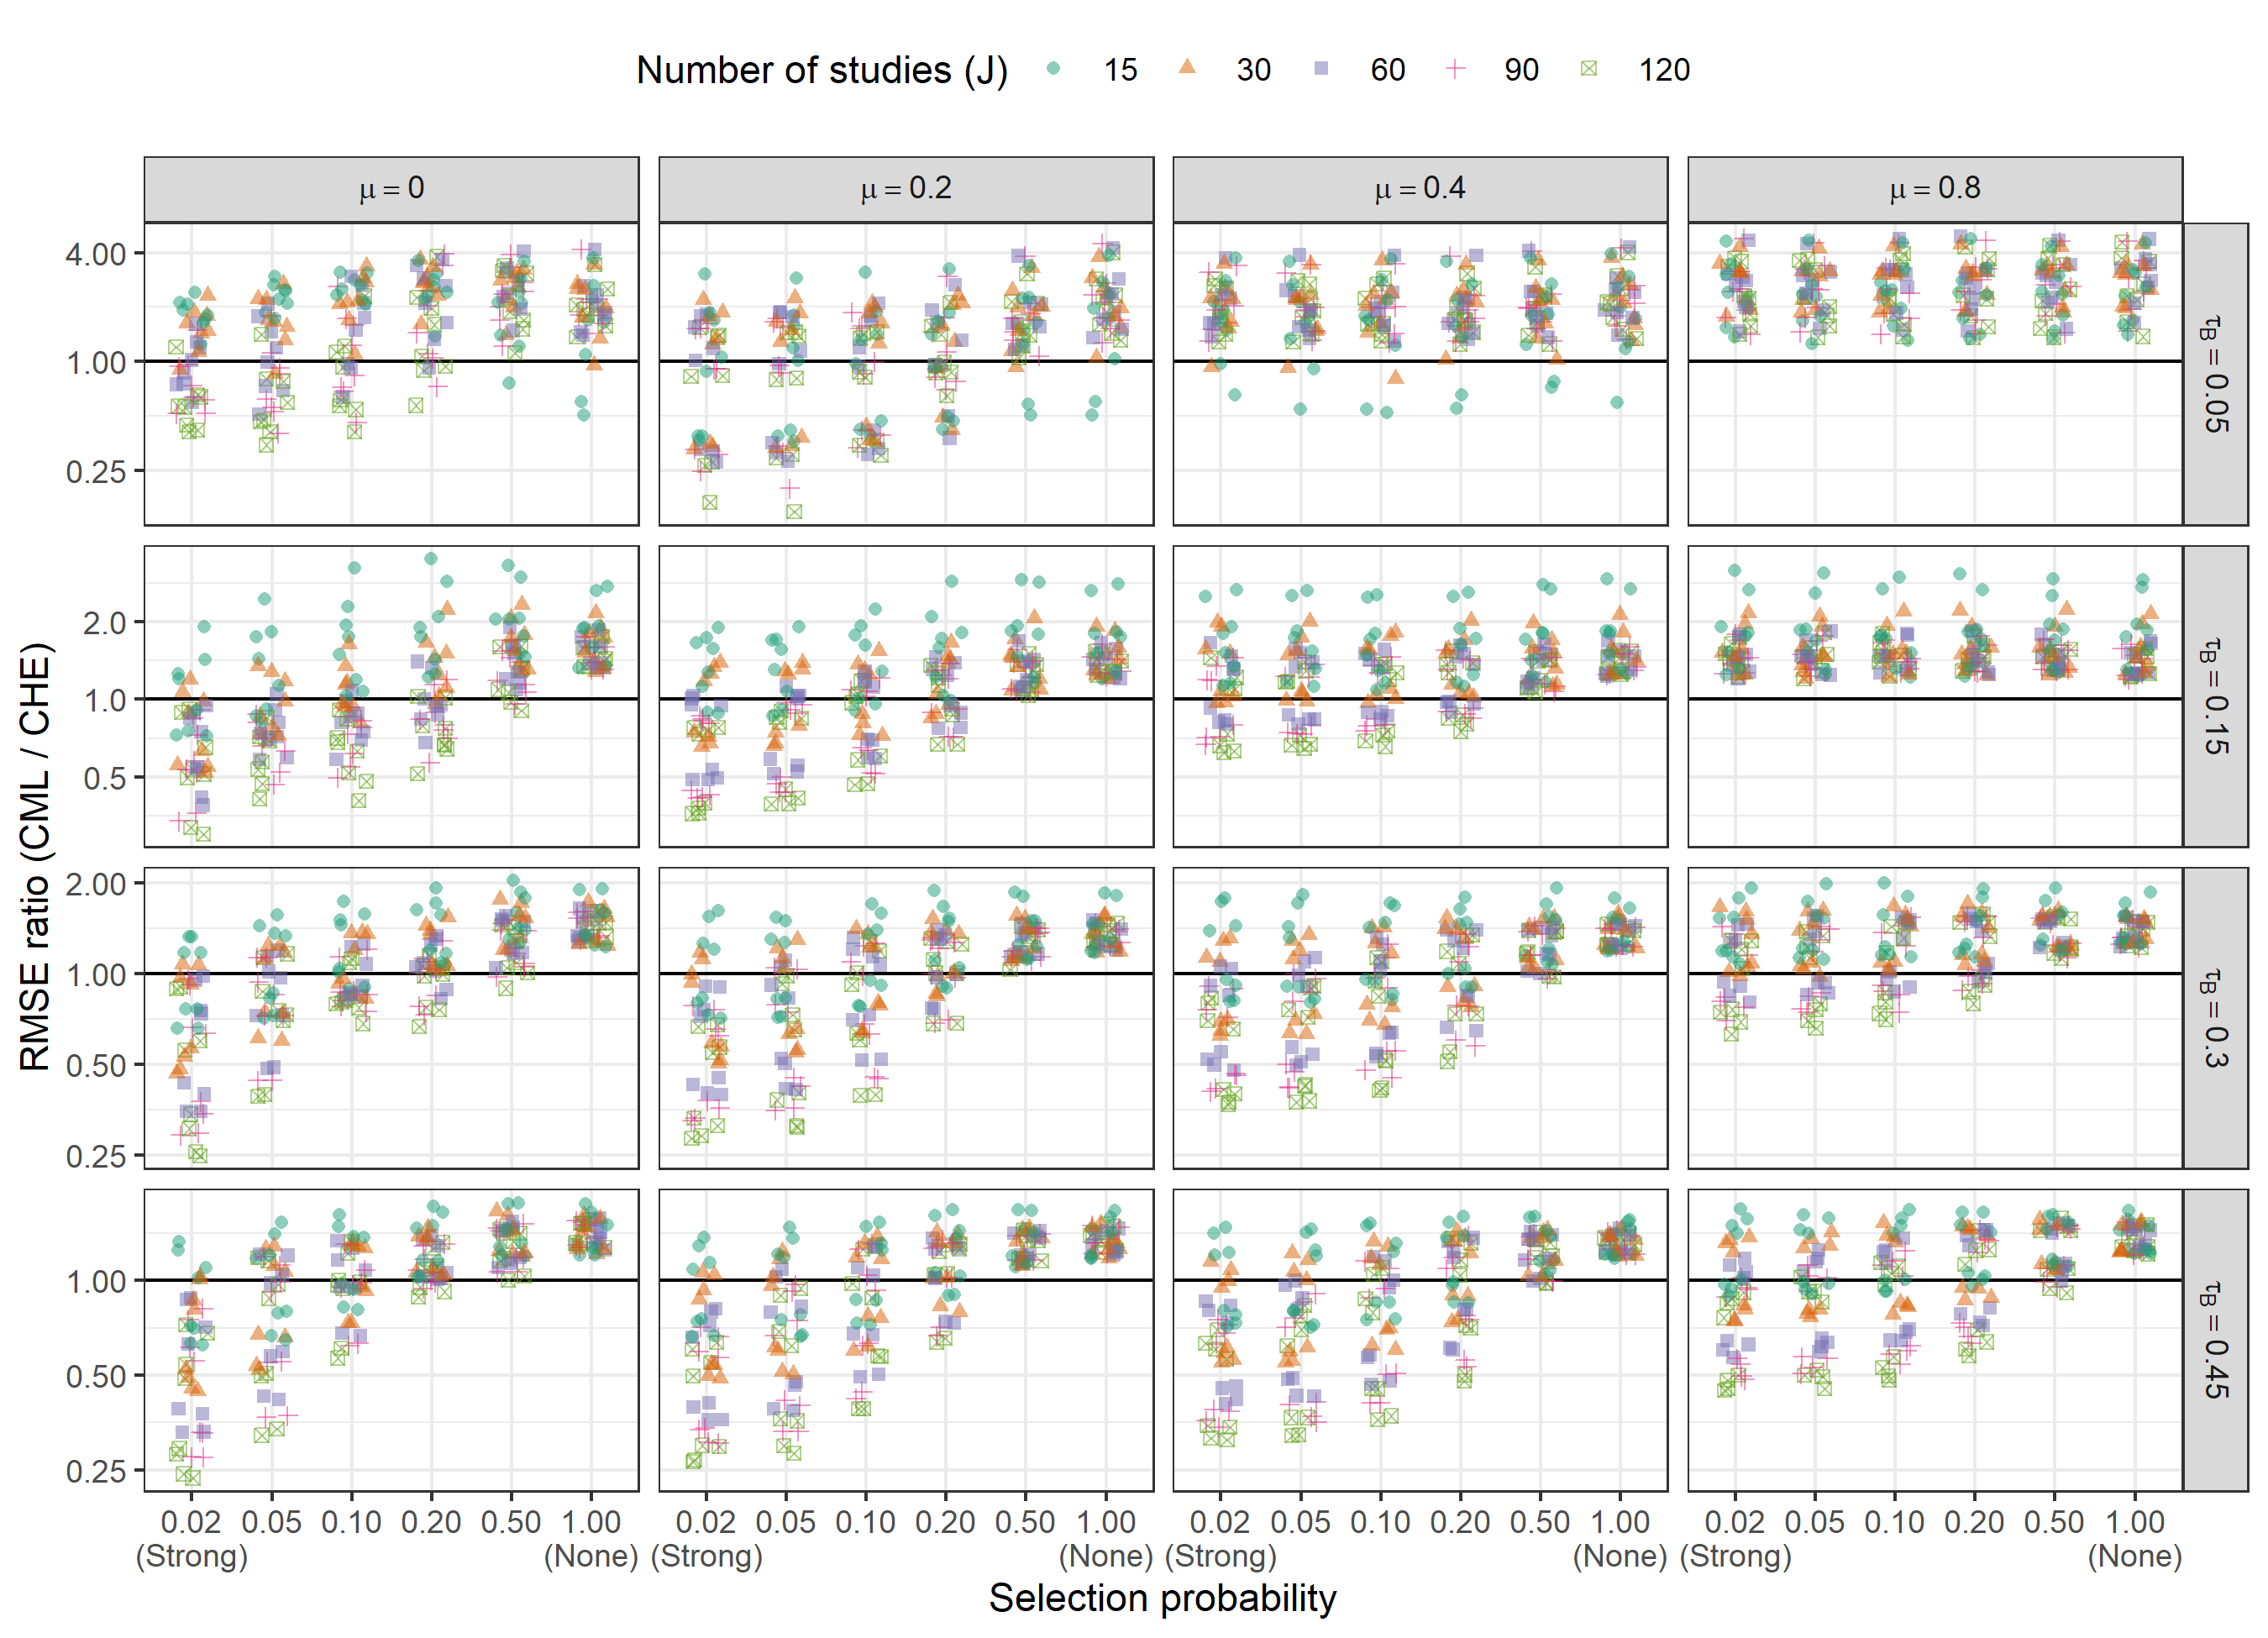
\includegraphics{step-function-selection-models-supplementary-materials_files/figure-latex/heterogeneity-rmse-CML-CHE-1} \caption{Ratio of root mean-squared error for CML heterogeneity estimator to root mean-squared error of CHE heterogeneity estimator by selection probability, number of studies, average SMD, and between-study heterogeneity}\label{fig:heterogeneity-rmse-CML-CHE}
\end{sidewaysfigure}

\begin{sidewaysfigure}
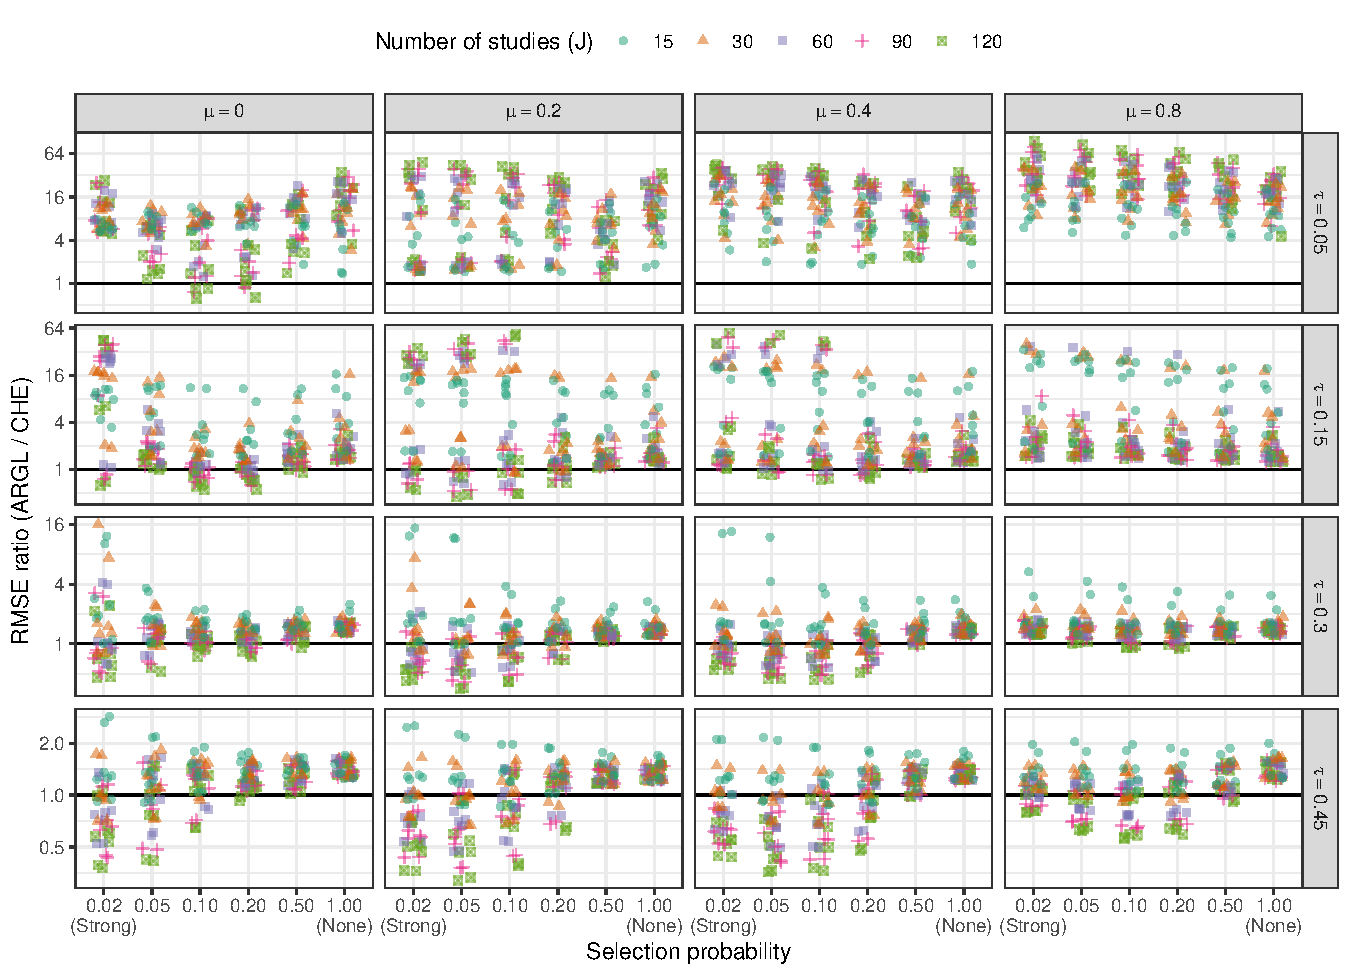
\includegraphics{step-function-selection-models-supplementary-materials_files/figure-latex/heterogeneity-rmse-ARGL-CHE-1} \caption{Ratio of root mean-squared error for ARGL heterogeneity estimator to root mean-squared error of CHE heterogeneity estimator by selection probability, number of studies, average SMD, and between-study heterogeneity}\label{fig:heterogeneity-rmse-ARGL-CHE}
\end{sidewaysfigure}

\begin{sidewaysfigure}
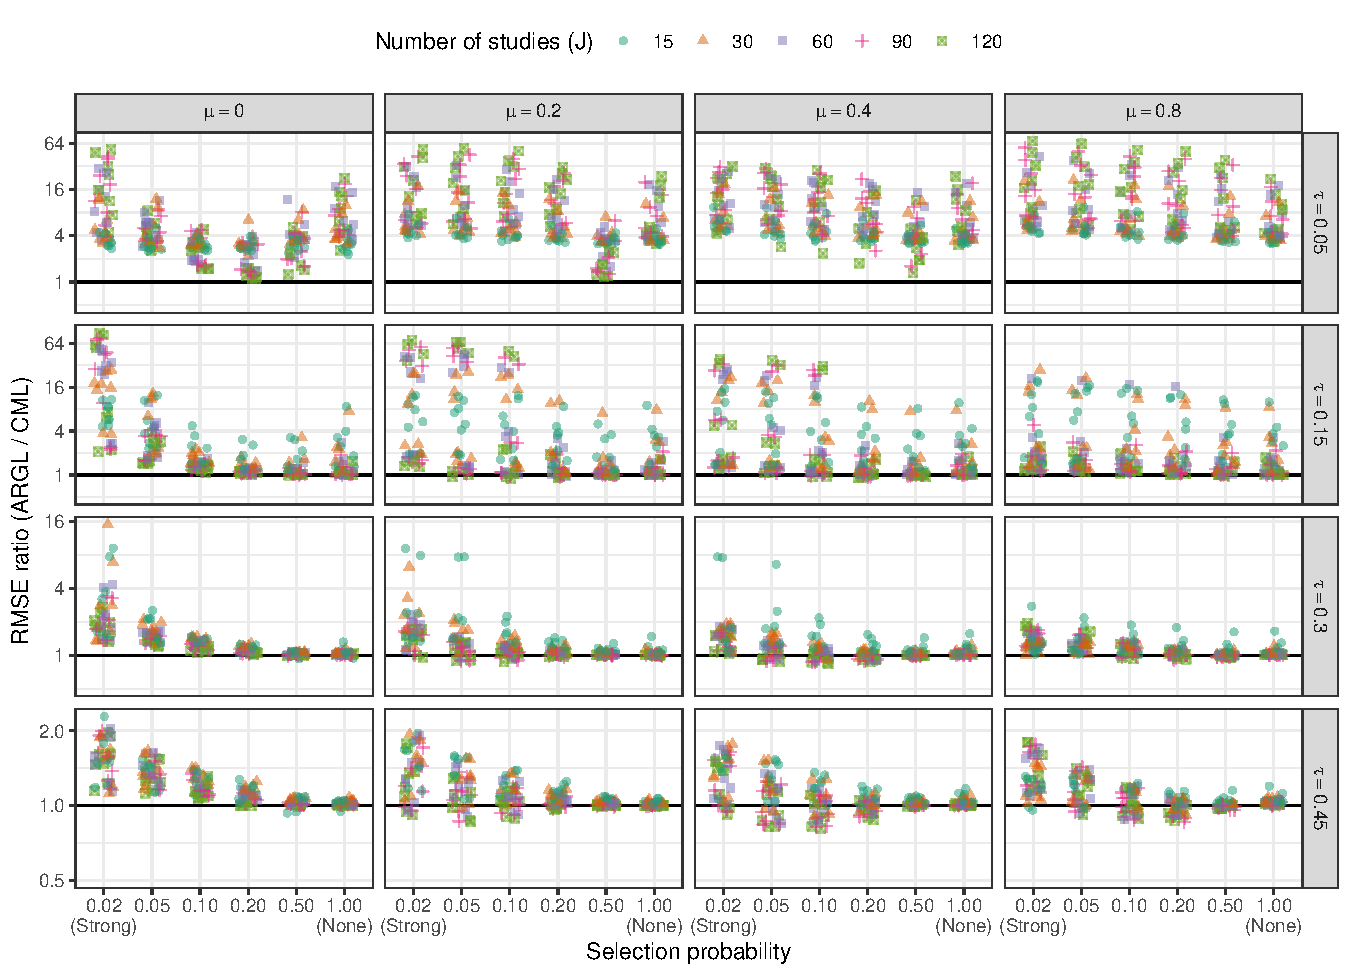
\includegraphics{step-function-selection-models-supplementary-materials_files/figure-latex/heterogeneity-rmse-ARGL-CML-1} \caption{Ratio of root mean-squared error for ARGL heterogeneity estimator to root mean-squared error of CML heterogeneity estimator by selection probability, number of studies, average SMD, and between-study heterogeneity}\label{fig:heterogeneity-rmse-ARGL-CML}
\end{sidewaysfigure}

\section{\texorpdfstring{Additional simulation results for estimators of selection parameter \((\zeta_1)\)}{Additional simulation results for estimators of selection parameter (\textbackslash zeta\_1)}}\label{zeta-simulation-results}

\begin{sidewaysfigure}
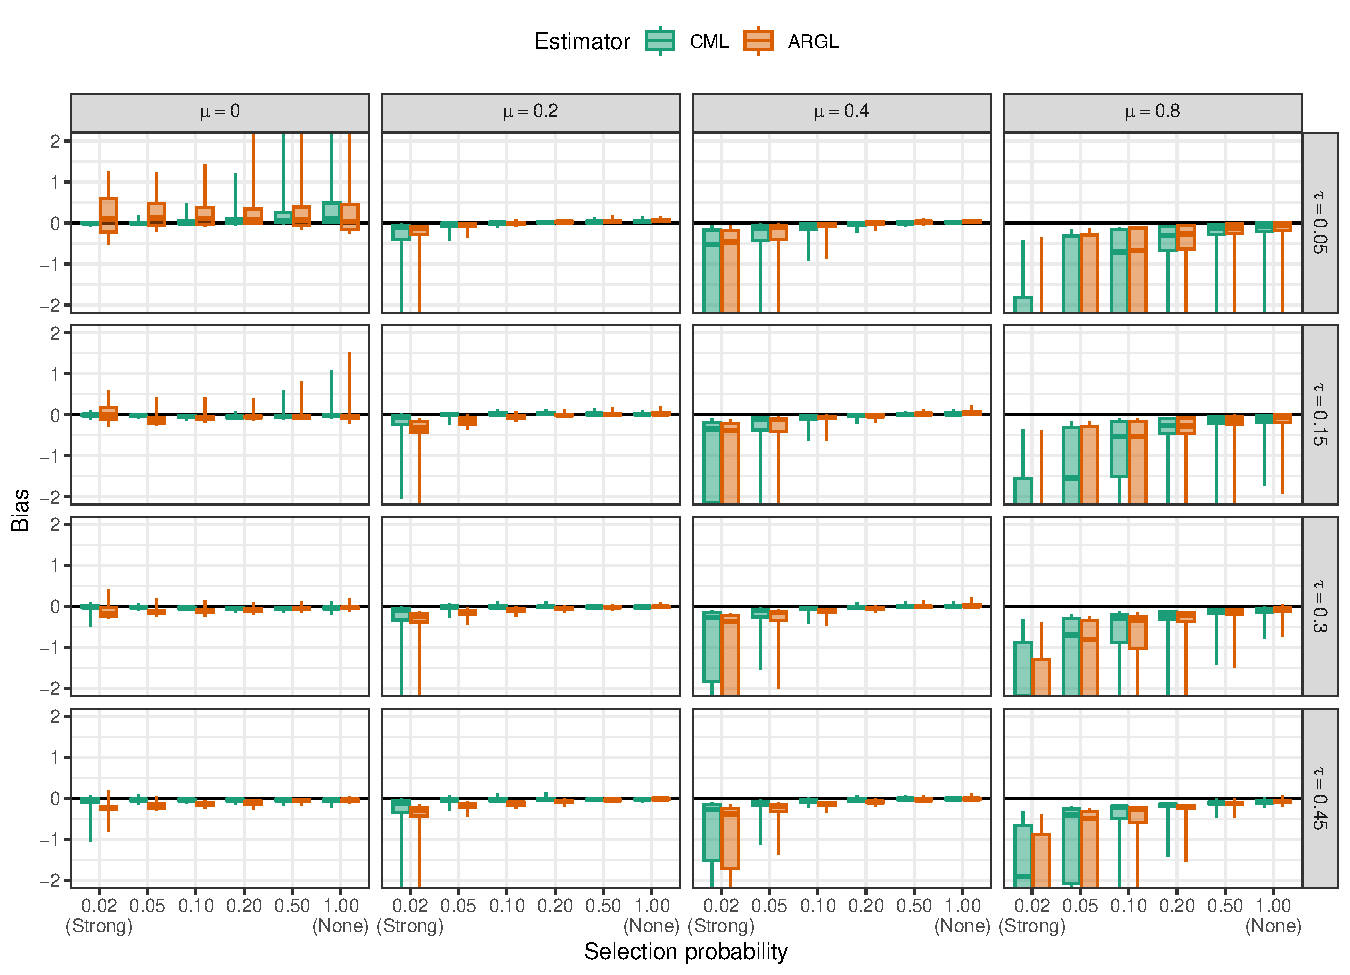
\includegraphics{step-function-selection-models-supplementary-materials_files/figure-latex/selection-bias-1} \caption{Bias for estimators of log-selection parameter by selection probability, average SMD, and between-study heterogeneity}\label{fig:selection-bias}
\end{sidewaysfigure}

\begin{sidewaysfigure}
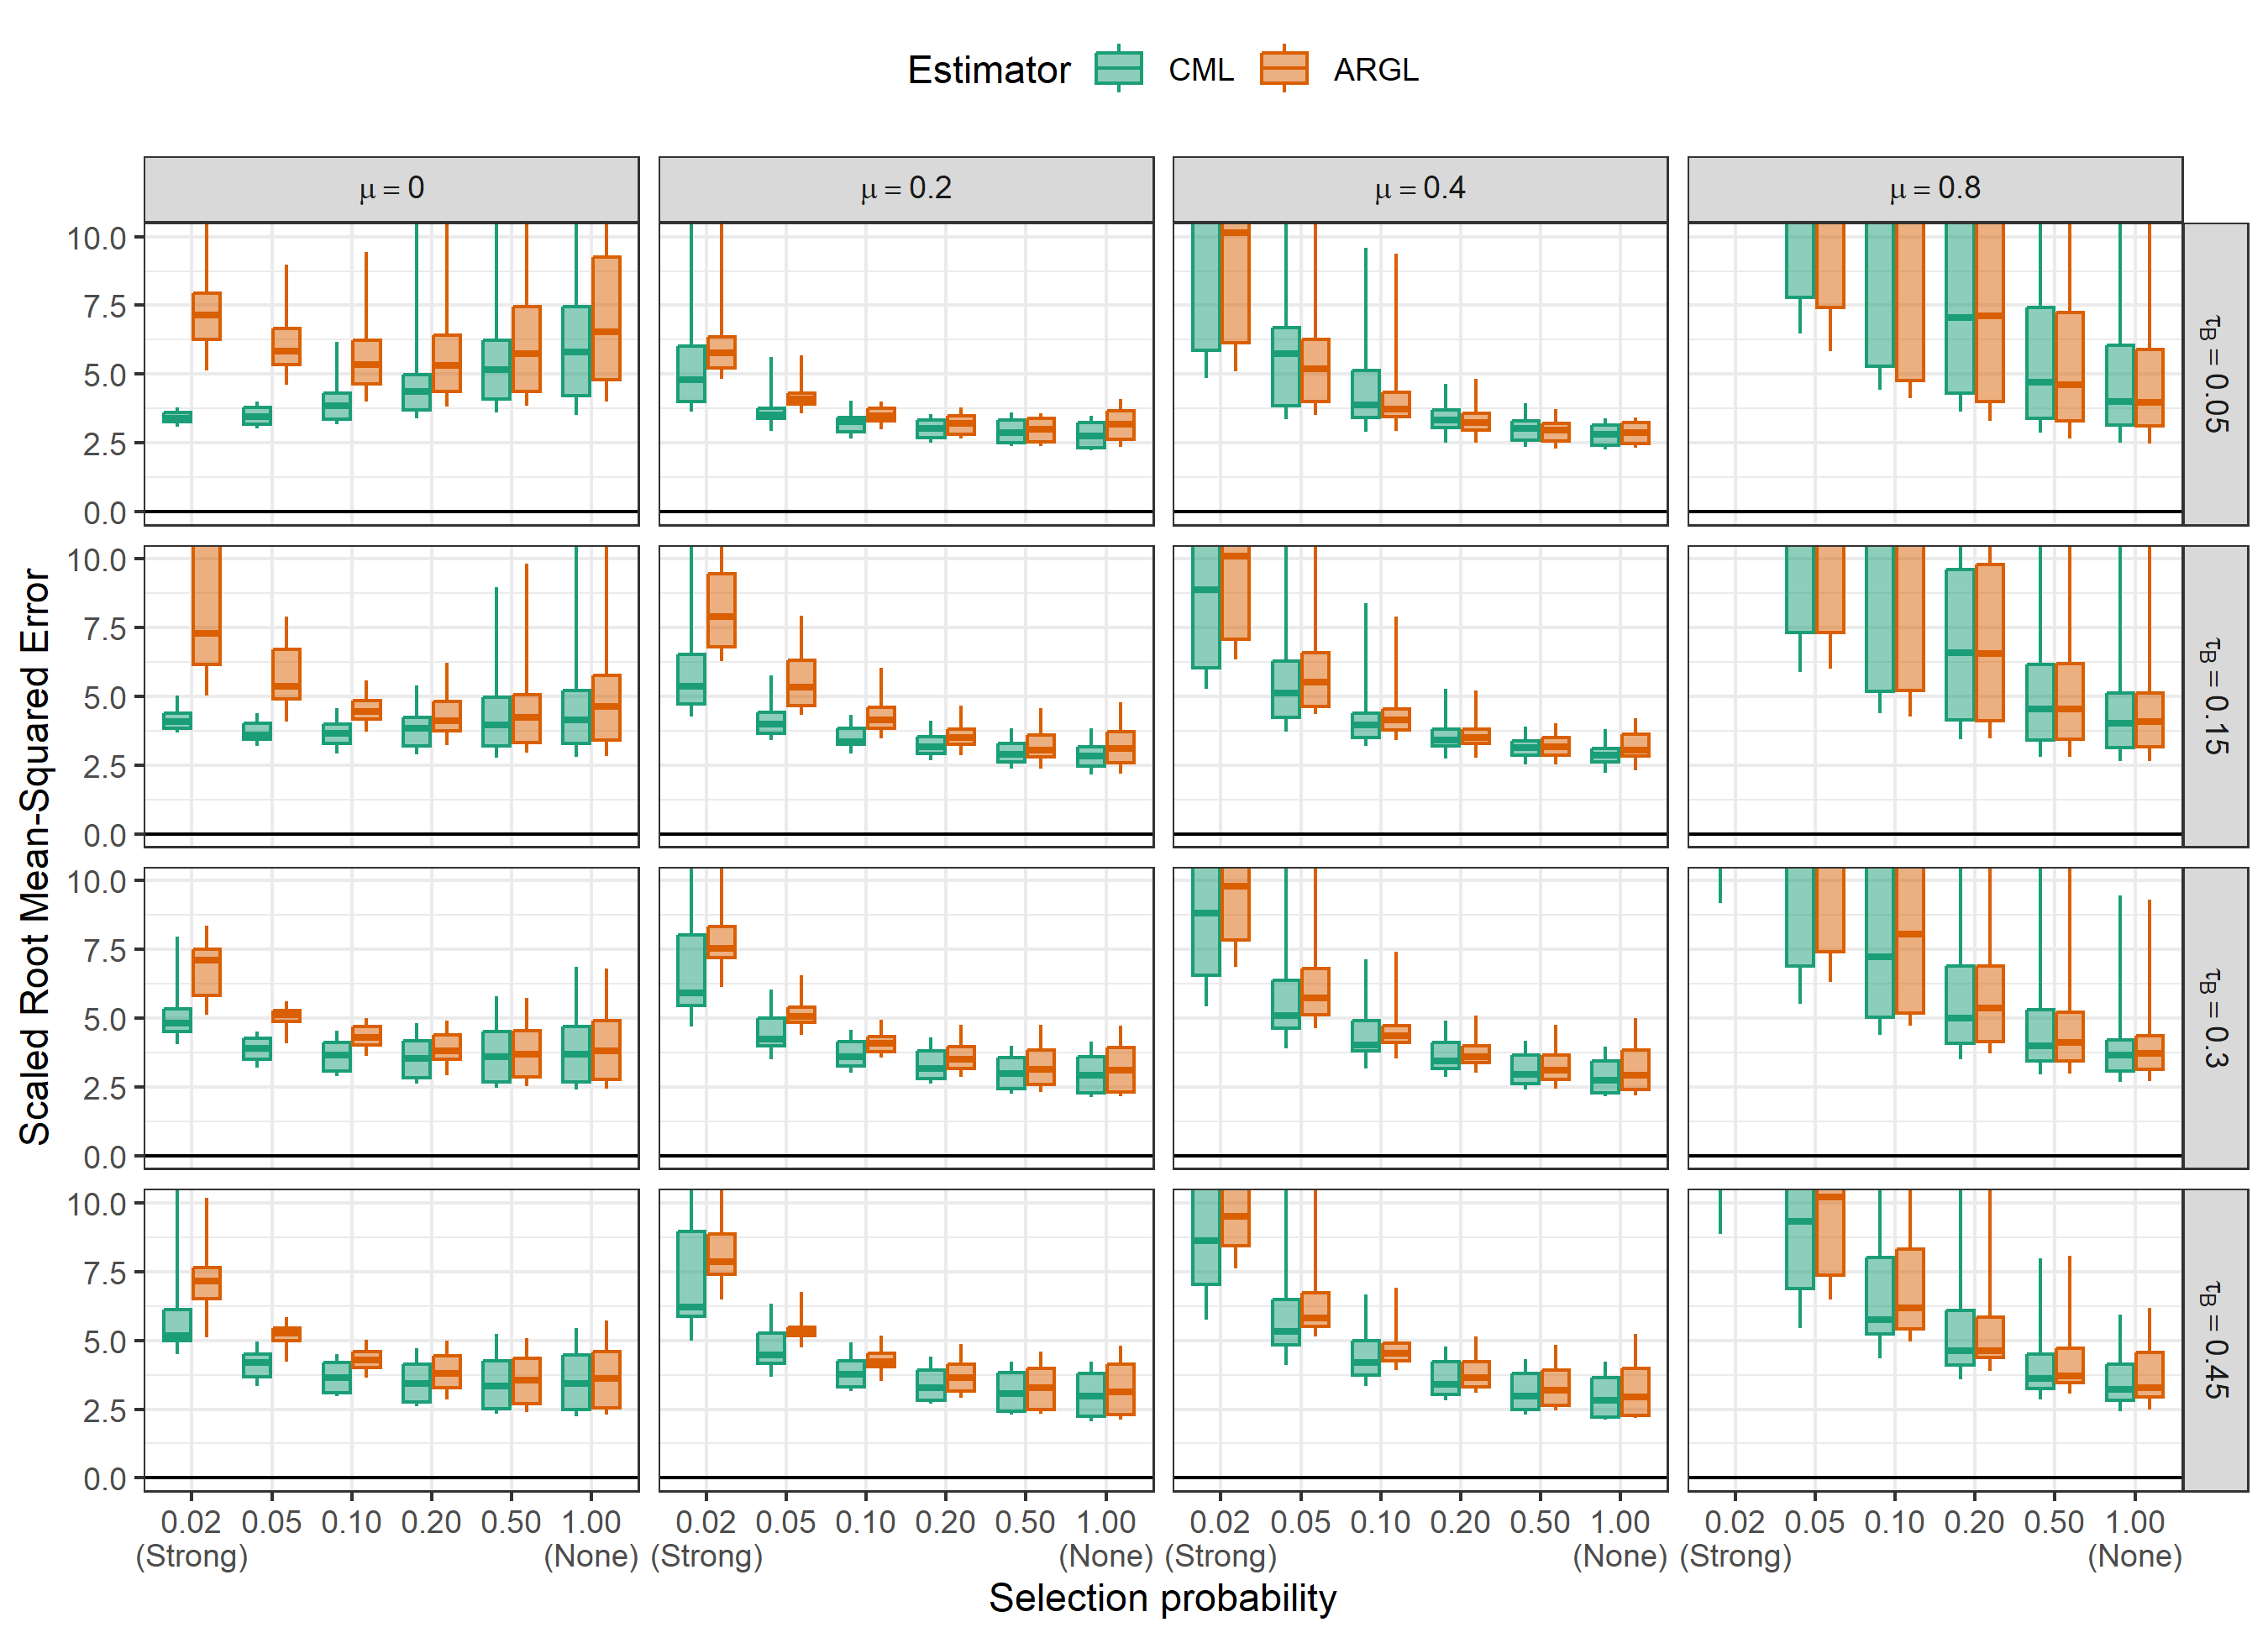
\includegraphics{step-function-selection-models-supplementary-materials_files/figure-latex/selection-rmse-1} \caption{Scaled root mean-squared error for log-selection parameter estimators by selection probability, average SMD, and between-study heterogeneity}\label{fig:selection-rmse}
\end{sidewaysfigure}

\begin{sidewaysfigure}
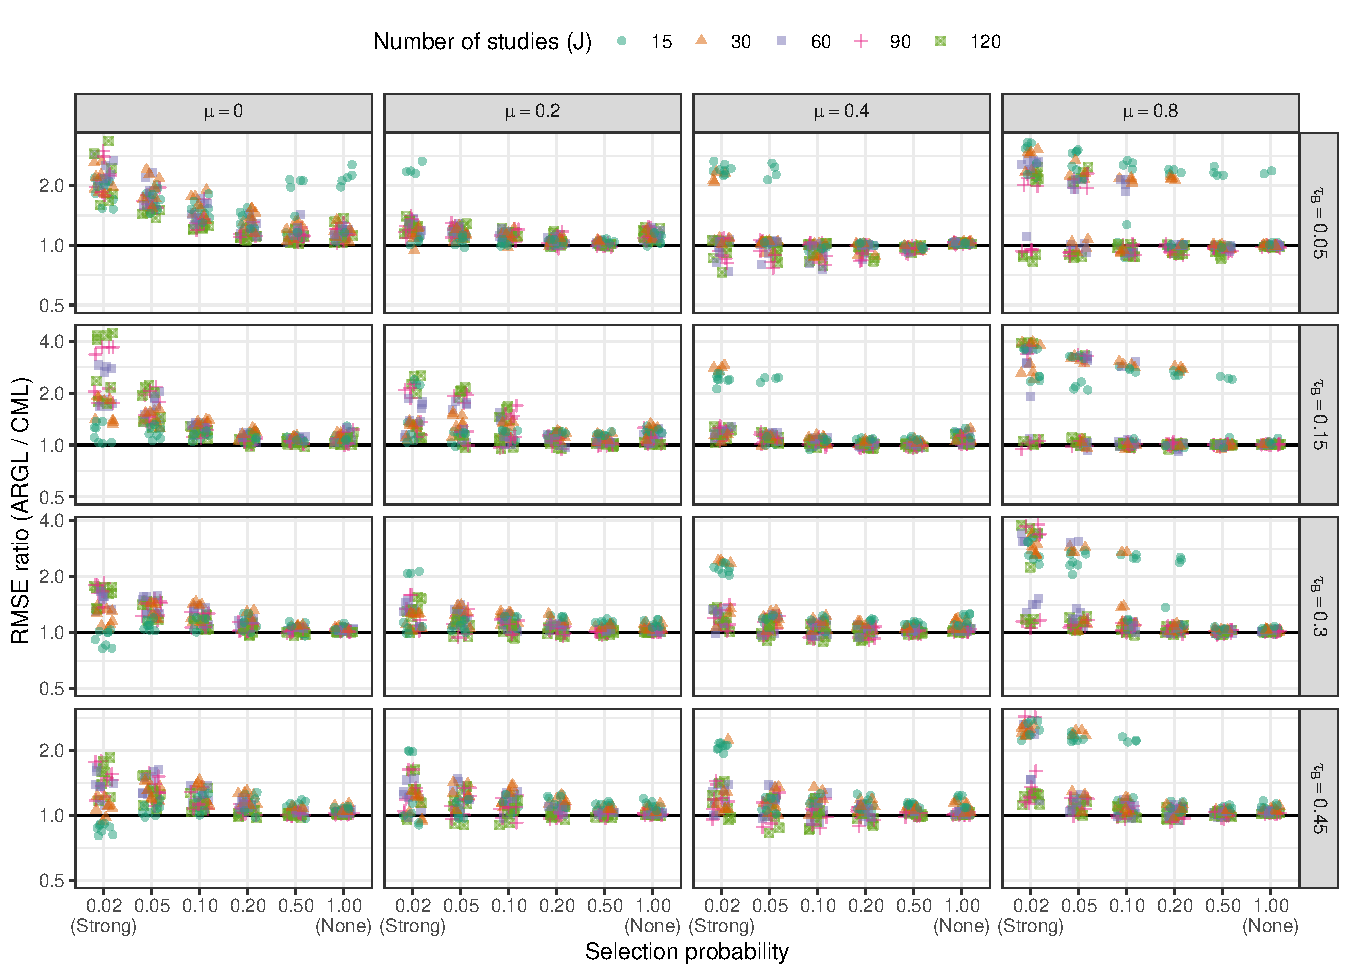
\includegraphics{step-function-selection-models-supplementary-materials_files/figure-latex/selection-rmse-ARGL-CML-1} \caption{Ratio of root mean-squared error for ARGL log-selection parameter estimator to root mean-squared error of CML log-selection parameter estimator by selection probability, number of studies, average SMD, and between-study heterogeneity}\label{fig:selection-rmse-ARGL-CML}
\end{sidewaysfigure}

\begin{sidewaysfigure}
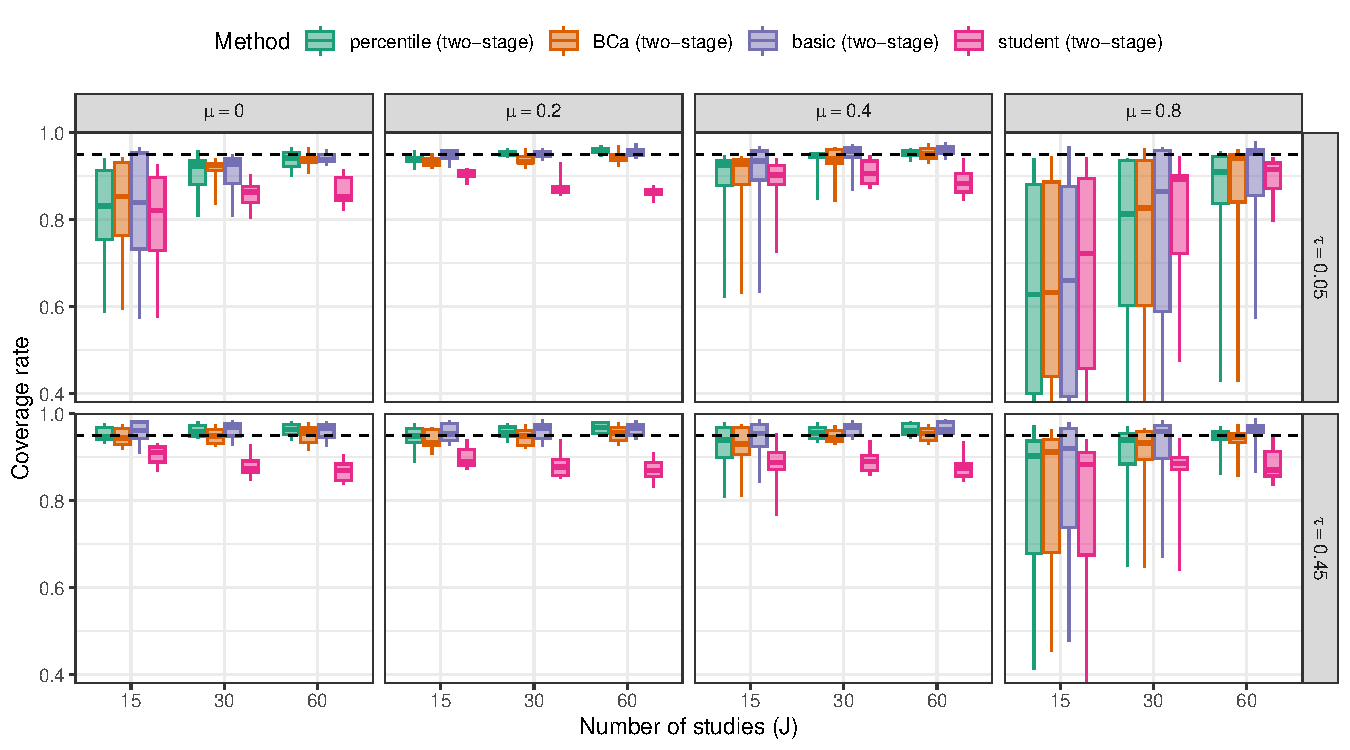
\includegraphics{step-function-selection-models-supplementary-materials_files/figure-latex/CML-zeta-coverage-two-stage-1} \caption{Coverage levels of two-stage bootstrap confidence intervals based on the CML estimator of log-selection parameter by number of studies, average SMD, and between-study heterogeneity. Dashed lines correspond to the nominal confidence level of 0.95.}\label{fig:CML-zeta-coverage-two-stage}
\end{sidewaysfigure}

\begin{sidewaysfigure}
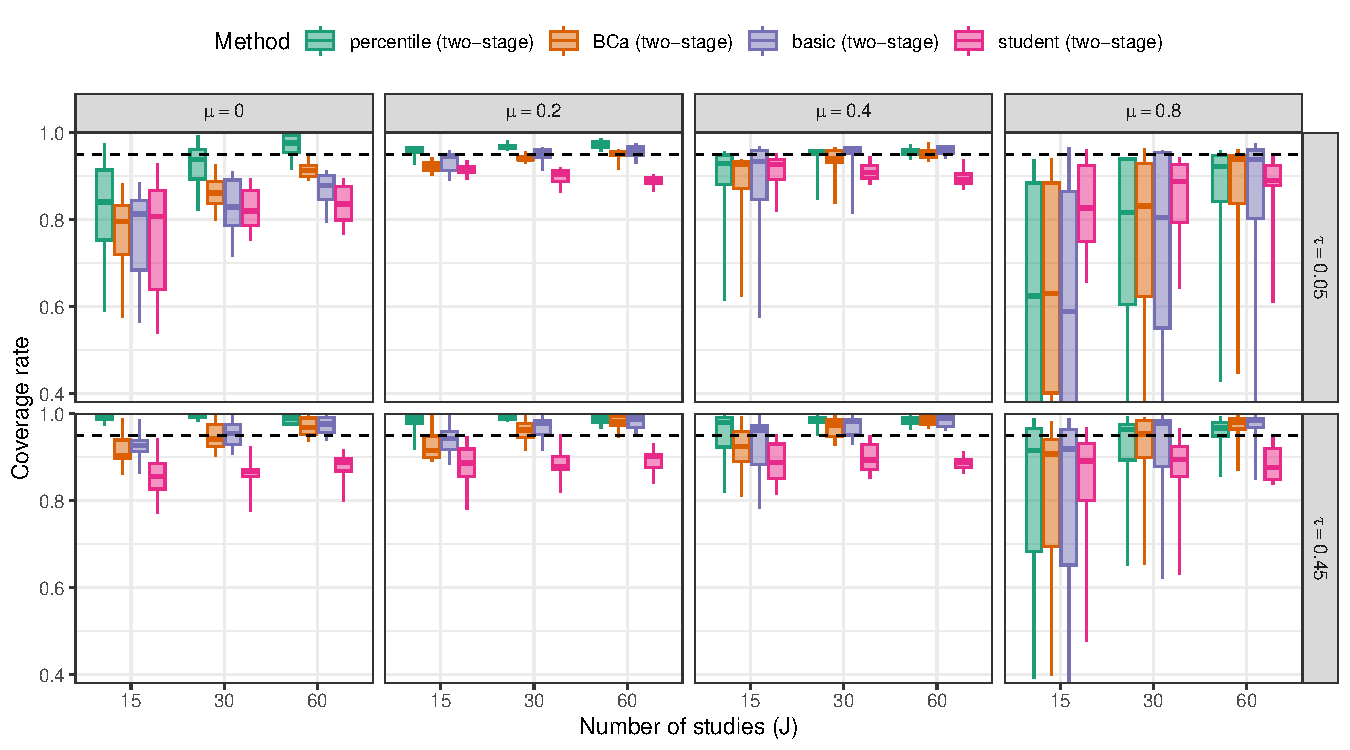
\includegraphics{step-function-selection-models-supplementary-materials_files/figure-latex/ARGL-zeta-coverage-two-stage-1} \caption{Coverage levels of two-stage bootstrap confidence intervals based on the ARGL estimator of log-selection parameter by number of studies, average SMD, and between-study heterogeneity. Dashed lines correspond to the nominal confidence level of 0.95.}\label{fig:ARGL-zeta-coverage-two-stage}
\end{sidewaysfigure}
\newpage

\section*{Additional References}\label{additional-references}
\addcontentsline{toc}{section}{Additional References}

\begingroup
\setlength{\parindent}{-0.5in}

\protect\phantomsection\label{refs}
\begin{CSLReferences}{0}{1}
\bibitem[\citeproctext]{ref-xu2020applications}
\CSLLeftMargin{1. }%
\CSLRightInline{Xu L, Gotwalt C, Hong Y, King CB, Meeker WQ. Applications of the fractional-random-weight bootstrap. \emph{The American Statistician}. 2020;74(4):345-358. doi:\href{https://doi.org/10.1080/00031305.2020.1731599}{10.1080/00031305.2020.1731599}}

\end{CSLReferences}

\endgroup


\end{document}
